\documentclass[journal]{IEEEtran}

\usepackage{iftex}
\ifPDFTeX
  \usepackage[utf8]{inputenc}
  \usepackage[T1]{fontenc}
\fi

\usepackage{cite}
\usepackage{amsmath,amssymb,amsfonts}
\usepackage{algorithmic}
\usepackage{graphicx}
\usepackage{textcomp}
\usepackage{xcolor}
\usepackage{adjustbox}
\usepackage{multirow}
\usepackage{booktabs}
\usepackage{makecell}
\usepackage{bm}
\usepackage{url}
\usepackage[hidelinks,hypertexnames=false]{hyperref}
\usepackage{dblfloatfix}
\usepackage{placeins}
\usepackage{tikz}
\usetikzlibrary{arrows.meta,positioning,fit,backgrounds,calc,decorations.pathreplacing}

\setlength{\emergencystretch}{1em}

% Math and Model Macros
\newcommand{\HSL}{\textit{HaarSymLite}}
\newcommand{\RRN}{\textit{ResRR-Net}}
\newcommand{\DWT}{\mathrm{DWT}}
\newcommand{\IDWT}{\mathrm{IDWT}}
\newcommand{\best}[1]{\textbf{#1}}
\newcommand{\second}[1]{\underline{#1}}

\begin{document}

\title{HaarSymLite: Lightweight 1D Wavelet Residual Network for High-Fidelity ECG Denoising and Downstream Arrhythmia Classification}

\author{Nguyen Dao Nam Hai, Dang Trung Khanh, Huy-Dung Han, and Loan Pham-Nguyen%
\thanks{Nguyen Dao Nam Hai and Dang Trung Khanh are with the School of Information and Communication Technology and the School of Electrical and Electronic Engineering, Hanoi University of Science and Technology (HUST), Hanoi, Vietnam.}%
\thanks{Huy-Dung Han and Loan Pham-Nguyen are with the School of Electrical and Electronic Engineering, Hanoi University of Science and Technology (HUST), Hanoi, Vietnam (e-mail: loan.phamnguyenthanh@hust.edu.vn).}%
\thanks{This research was conducted at the SPARC Laboratory and Biomedical Electronics Laboratory (BME Lab), Hanoi University of Science and Technology (HUST).}%
}

% \markboth{IEEE Transactions on Biomedical Engineering / Biomedical Signal Processing and Control,~Vol.~XX, No.~X, October~2026}%
% {Hai \MakeLowercase{\textit{et al.}}: HaarSymLite: Lightweight 1D Wavelet Residual Network for ECG Denoising and Classification}

\maketitle

% Modular Section Inputs
\begin{abstract}
Electrocardiogram (ECG) denoising plays a vital role in mobile health and wearable monitoring, where real-world recordings are heavily corrupted by baseline wander (BW), muscle artifacts (MA), and electrode motion (EM). While conventional deep denoising networks achieve substantial noise suppression, they frequently cause diagnostic distortion by blunting high-frequency QRS complexes and attenuating weak P/T waves. Furthermore, denoising models are rarely validated on downstream clinical diagnosis under standardized inter-patient protocols. In this paper, we propose \HSL, an ultra-lightweight 75{,}133-parameter one-dimensional wavelet residual network designed for morphology-preserving ECG reconstruction and automated arrhythmia detection. \HSL{} integrates discrete Haar wavelet decomposition directly into a symmetric U-Net backbone with standard residual blocks with squeeze-and-excitation channel attention (\texttt{ResSEBlock1D}), and high-frequency detail subband residual filtering. To prevent R-peak clipping and baseline distortion, the network is trained with a time-domain mixed loss objective combining mean squared error and absolute error ($\alpha=0.8$). For downstream arrhythmia classification, we introduce \RRN, which couples a 1D ResNet morphology encoder (with SiLU activations) with an independent 6-dimensional RR-interval contextual pathway and interchangeable classical MLP or 6-qubit parameterized variational quantum circuit (VQC) classification heads. Evaluated on the MIT-BIH Arrhythmia Database paired with NSTDB physiological noise across 7 noise combinations and 10 SNR levels ($-10$ to $+10$\,dB), \HSL{} achieves an average SNR improvement ($\Delta$SNR) of \best{10.01\,dB} and a percentage root-mean-square difference (PRD) of \best{33.88\%}, outperforming recent SOTA DeepFilter (9.64\,dB / 35.63\%) and four baseline architectures while requiring only 35.20\,ms inference time on edge CPU. On the clinical gold-standard de Chazal inter-patient DS1/DS2 test split comprising 49{,}298 independent beats from 22 unseen subjects, the downstream classifier achieves an Accuracy of \best{96.43\%}, a Macro-F1 score of \best{0.8407}, and an S-class positive predictivity of \best{72.97\%} (+23.27 percentage points over prior benchmarks) (Classical ensemble) and \best{96.04\%} / \best{0.8176} (Hybrid quantum ensemble). Ablation studies demonstrate that channel-wise attention (SE1D) preserves high-frequency QRS morphology substantially better than spatial attention (CBAM1D), providing an efficient and reliable foundation for wearable cardiac monitoring.
\end{abstract}

\begin{IEEEkeywords}
Electrocardiogram (ECG) denoising, discrete wavelet transform (DWT), squeeze-and-excitation, heartbeat classification, variational quantum circuit (VQC), inter-patient evaluation, wearable edge computing.
\end{IEEEkeywords}

\section{Introduction}
\label{sec:intro}

The electrocardiogram (ECG) represents the primary non-invasive diagnostic modality for assessing cardiac electrophysiology and detecting cardiovascular diseases (CVDs), which remain the leading cause of global mortality \cite{clifford2006}. In recent years, continuous cardiac monitoring has undergone a paradigm shift from specialized hospital environments toward ambulatory and wearable consumer electronics, such as smartwatches, Holter patches, and chest straps. However, in mobile and unconstrained settings, acquired ECG signals are intrinsically vulnerable to multiple sources of physiological and environmental contamination \cite{clifford2006,jin2024}. The most prevalent artifacts include baseline wander (BW), induced by respiration and thoracic impedance variations ($0.05$--$1$\,Hz); muscle artifacts (MA), generated by skeletal muscle contraction ($5$--$50$\,Hz); and electrode motion (EM), caused by movement between the skin and sensor interface. Because MA and EM artifacts overlap significantly with the diagnostic frequency bands of the P-wave, QRS complex, and T-wave, simple frequency-domain filtering cannot isolate noise without corrupting essential clinical wave morphologies.

To address non-stationary cardiac noise, traditional techniques such as digital bandpass filters, adaptive filtering, empirical mode decomposition (EMD), and discrete wavelet thresholding have been extensively utilized \cite{clifford2006,goldberger2000}. Although computationally inexpensive, these classical approaches depend heavily on handcrafted heuristic rules, mother wavelet selection, and static thresholding policies. Consequently, aggressive filtering frequently suppresses low-amplitude diagnostic waveforms (such as P-wave onset or subtle ST-segment deviations) or induces non-linear phase shifts that distort the spatial positioning of R-peaks.

\begin{figure*}[!t]
\centering
\begin{adjustbox}{max width=0.98\textwidth}
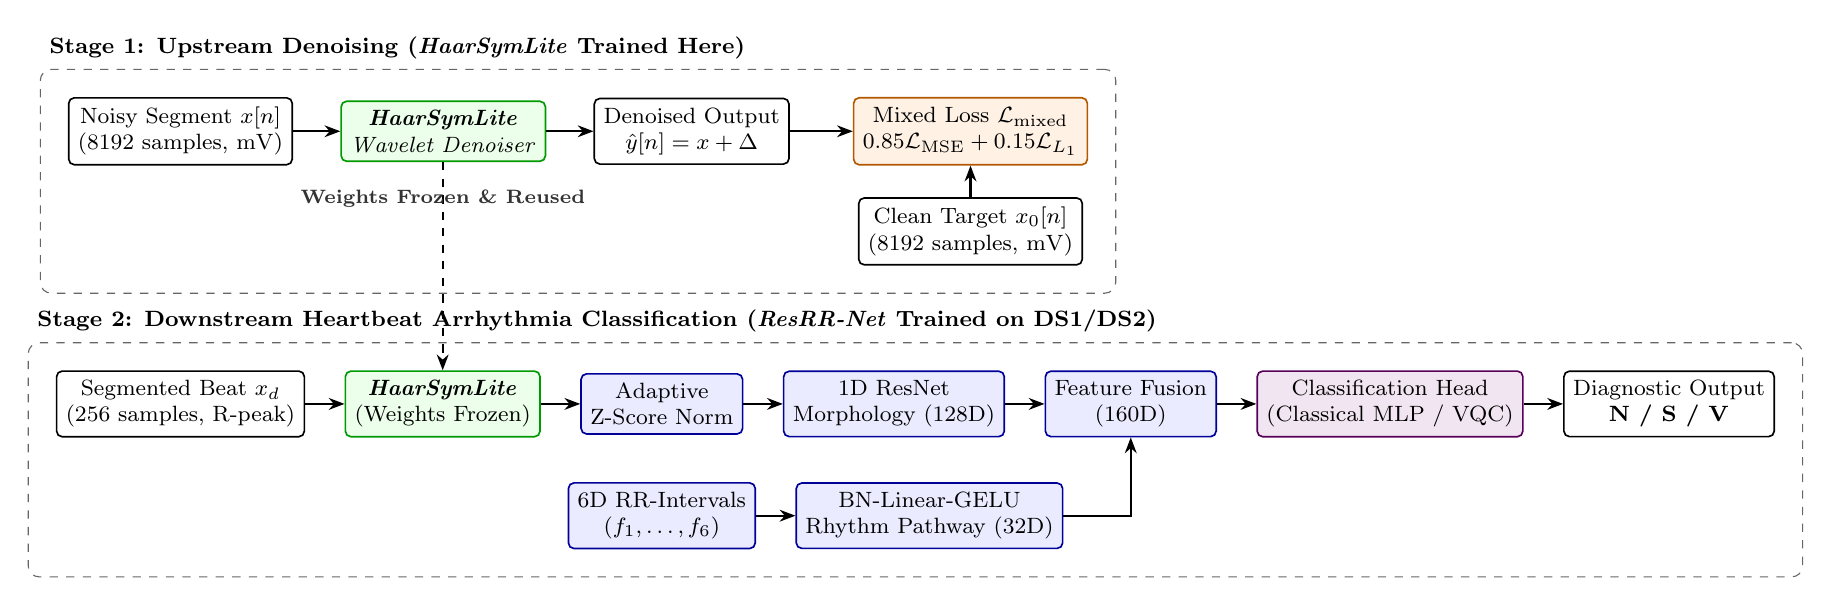
\begin{tikzpicture}[
  node distance=4mm,
  blk/.style={draw, rectangle, rounded corners=2pt, minimum height=7mm, minimum width=1.4cm, align=center, font=\footnotesize, fill=white, line width=0.6pt},
  den/.style={blk, fill=green!8, draw=green!60!black},
  cls/.style={blk, fill=blue!8, draw=blue!60!black},
  qnt/.style={blk, fill=violet!10, draw=violet!70!black},
  lossn/.style={blk, fill=orange!10, draw=orange!70!black},
  arr/.style={-{Stealth[length=2mm]}, thick},
  darr/.style={-{Stealth[length=2mm]}, thick, dashed},
  grp/.style={draw=black!60, dashed, rounded corners=4pt, inner sep=3.5mm, font=\scriptsize\bfseries}
]

% ==================== STAGE 1 ====================
\node[blk] (n1) {Noisy Segment $x[n]$\\($8192$ samples, $\mathrm{mV}$)};
\node[den, right=6mm of n1] (n2) {\textbf{\HSL}\\\textit{Wavelet Denoiser}};
\node[blk, right=6mm of n2] (n3) {Denoised Output\\$\hat{y}[n] = x + \Delta$};
\node[lossn, right=8mm of n3] (ls) {Mixed Loss $\mathcal{L}_{\mathrm{mixed}}$\\$0.85\mathcal{L}_{\mathrm{MSE}} + 0.15\mathcal{L}_{L_1}$};
\node[blk, below=4mm of ls] (n4) {Clean Target $x_0[n]$\\($8192$ samples, $\mathrm{mV}$)};

\draw[arr] (n1) -- (n2);
\draw[arr] (n2) -- (n3);
\draw[arr] (n3) -- (ls);
\draw[arr] (n4) -- (ls);

\begin{scope}[on background layer]
\node[grp, fit=(n1)(n2)(n3)(ls)(n4), label={[font=\footnotesize\bfseries, anchor=south west]north west:\textbf{Stage 1: Upstream Denoising (\HSL{} Trained Here)}}] (g1) {};
\end{scope}

% ==================== STAGE 2 ====================
\node[blk, below=26mm of n1] (m1) {Segmented Beat $x_d$\\($256$ samples, R-peak)};
\node[den, right=5mm of m1] (m2) {\textbf{\HSL}\\(Weights Frozen)};
\node[cls, right=5mm of m2] (m3) {Adaptive\\Z-Score Norm};
\node[cls, right=5mm of m3] (m4) {1D ResNet\\Morphology (128D)};
\node[cls, right=5mm of m4] (m5) {Feature Fusion\\(160D)};
\node[qnt, right=5mm of m5] (m6) {Classification Head\\(Classical MLP / VQC)};
\node[blk, right=5mm of m6] (m7) {Diagnostic Output\\\textbf{N / S / V}};

% RR Context Branch
\node[cls, below=6mm of m3] (r1) {6D RR-Intervals\\($f_1, \dots, f_6$)};
\node[cls, right=5mm of r1] (r2) {BN-Linear-GELU\\Rhythm Pathway (32D)};

\draw[arr] (m1) -- (m2);
\draw[arr] (m2) -- (m3);
\draw[arr] (m3) -- (m4);
\draw[arr] (m4) -- (m5);
\draw[arr] (m5) -- (m6);
\draw[arr] (m6) -- (m7);

\draw[arr] (r1) -- (r2);
\draw[arr] (r2.east) -| (m5.south);

% Frozen weights arrow
\draw[darr] (n2.south) -- ++(0,-7mm) -| node[pos=0.25, above, font=\scriptsize\bfseries, text=black!80]{Weights Frozen \& Reused} (m2.north);

\begin{scope}[on background layer]
\node[grp, fit=(m1)(m2)(m7)(r1)(r2), label={[font=\footnotesize\bfseries, anchor=south west]north west:\textbf{Stage 2: Downstream Heartbeat Arrhythmia Classification (\RRN{} Trained on DS1/DS2)}}] (g2) {};
\end{scope}

\end{tikzpicture}
\end{adjustbox}
\caption{End-to-end framework for wearable ECG analysis. \textbf{Stage 1 (Top)}: \HSL{} is trained on 8192-sample raw-scale continuous segments under single and multi-source NSTDB noise with a physics-preserving mixed objective. \textbf{Stage 2 (Bottom)}: The frozen denoiser purifies segmented 256-sample cardiac beats, processed by \RRN{} alongside an independent 6-dimensional RR interval timing pathway. Dual interchangeable heads (Classical MLP and 6-qubit Hybrid VQC) perform final 3-class AAMI arrhythmia classification (N, S, V) on the 49{,}298-beat inter-patient DS2 test set.}
\label{fig:pipeline}
\end{figure*}

With the advent of deep learning, neural networks have demonstrated superior non-linear mapping capabilities by learning directly from data pairs \cite{vincent2008,chiang2019}. Denoising autoencoders (DAEs), fully convolutional networks (FCNs), and lightweight U-Nets \cite{ronneberger2015,xiong2016} have shown significant noise suppression. More recently, two-dimensional time-frequency representations, such as the short-time Fourier transform (STFT), have been explored to expose multi-scale spectral patterns. However, STFT-based models exhibit substantial computational redundancy due to overlapping analysis windows, and denoising magnitude spectrograms requires separate, computationally intensive phase-retrieval algorithms (e.g., Griffin-Lim), which impedes real-time deployment on battery-constrained wearable edge devices \cite{jin2024}.

Hybrid architectures combining the discrete wavelet transform (DWT) with deep convolutional backbones offer an appealing compromise \cite{jin2024,nguyen2026liwave,nguyen2026dwse}. By embedding invertible, orthogonal wavelet operations within the network, multiresolution subbands are extracted without phase ambiguity or spatial redundancy. Despite these advances, two fundamental shortcomings persist in the state of the art:
\begin{enumerate}
    \item \textbf{High-Frequency Subband Attenuation and Loss Distortion:} Conventional DWT-based models predominantly decompose only the low-frequency approximation branch ($cA$), leaving the high-frequency detail subbands ($cD$) coarsely resolved. Concurrently, standard networks are optimized using Mean Squared Error (MSE), which penalizes large amplitude deviations quadratically. In ECG processing, this causes catastrophic peak-blunting: the network minimizes overall variance by smoothing the sharp R-peak and blunting the steep slopes of the QRS complex, compromising subsequent clinical analysis.
    \item \textbf{Disconnection from Downstream Arrhythmia Diagnosis:} The vast majority of ECG denoising studies evaluate performance exclusively using generic reconstruction metrics, such as Signal-to-Noise Ratio improvement ($\Delta$SNR) and Percentage Root-Mean-Square Difference (PRD). However, a high mathematical $\Delta$SNR does not ensure clinical fidelity. Crucially, denoising models are rarely subjected to downstream arrhythmia classification under the strict de Chazal inter-patient protocol (DS1/DS2) \cite{dechazal2004}, leaving the clinical utility of deep denoisers unverified on unseen patients.
\end{enumerate}

To bridge this divide, this paper proposes an integrated, two-stage clinical ECG processing framework (Fig.~\ref{fig:pipeline}). In Stage~1, we introduce \textbf{\HSL}, an ultra-compact 75{,}133-parameter 1D wavelet residual network that integrates multi-scale Haar DWT/IDWT operators, unified standard residual blocks with squeeze-and-excitation (\texttt{ResSEBlock1D}) with SiLU activations, and high-frequency detail subband residual filtering, trained under a composite time-domain mixed loss objective. In Stage~2, we design \textbf{\RRN}, a downstream heartbeat classifier that takes beats denoised by the frozen \HSL{} model, extracts deep morphological representations via a 1D ResNet encoder (with SiLU activations), fuses an independent 6-dimensional RR contextual rhythm pathway, and evaluates both a classical MLP head and a 6-qubit parameterized variational quantum circuit (VQC) head.

The primary contributions of this work are summarized as follows:
\begin{itemize}
    \item \textbf{Lightweight Wavelet Denoiser (\HSL):} We engineer a 75.1\,K-parameter symmetric wavelet U-Net combining two-level Haar DWT resolution scaling with unified \texttt{ResSEBlock1D} attention and detail subband filtering. \HSL{} achieves an average $\Delta$SNR of \best{10.01\,dB} and PRD of \best{33.88\%} across comprehensive test conditions on MITDB and NSTDB, surpassing recent SOTA DeepFilter \cite{romero2021} (9.64\,dB) and LiWave \cite{nguyen2026liwave} (9.21\,dB) while running at 35.20\,ms per segment on edge CPU.
    \item \textbf{Fiducial-Preserving Mixed Loss Formulation:} We systematically investigate loss objectives and demonstrate that our time-domain mixed loss ($\alpha L_{\mathrm{MSE}} + (1-\alpha)L_{L_1}$, $\alpha=0.8$) prevents the R-peak blunting inherent to pure MSE training, reducing R-amplitude error to only 0.048\,mV and preserving QRS and QT interval durations under NeuroKit2 clinical evaluation.
    \item \textbf{Downstream Inter-Patient Clinical Validation (\RRN):} We couple the frozen denoiser to a downstream classifier and rigorously benchmark on the 49{,}298-beat inter-patient DS2 test set (22 completely unseen patients). Our 5-seed soft-voting ensemble attains \best{96.43\%} accuracy and \best{0.8407} Macro-F1, significantly elevating supraventricular ectopic beat (S-class) positive predictivity (+P) to \best{72.97\%} (+23.27 percentage points over Mond{\'e}jar-Guerra \emph{et al.} \cite{mondejar2019}).
    \item \textbf{Exploration of Hybrid Quantum Computing and Ablation Insights:} We construct and validate a 6-qubit, 24-parameter VQC classifier with classical residual bypass, achieving an ensemble Macro-F1 of \best{0.8176}. Through controlled ablations, we provide the biomedical insight that channel attention (SE1D) is structurally superior to spatial attention (CBAM1D) for 1D ECG waveforms.
\end{itemize}

The remainder of this article is structured as follows. Section~\ref{sec:related} reviews related work and provides a comprehensive taxonomic comparison. Section~\ref{sec:method} details the mathematical formulation of \HSL{} and \RRN. Section~\ref{sec:exp} describes the dataset, experimental configurations, and metrics. Section~\ref{sec:results} presents quantitative denoising benchmarks, morphology preservation, latency, and classification results. Section~\ref{sec:discussion} discusses biological implications, quantum modeling, and edge deployment trade-offs. Section~\ref{sec:conclusion} concludes the paper.

\section{Related Work}
\label{sec:related}

\subsection{Traditional Filtering and Wavelet Thresholding}
Early research on ECG signal enhancement focused predominantly on digital finite/infinite impulse response (FIR/IIR) filters, adaptive noise cancelers based on least mean squares (LMS), and recursive Bayesian estimation (extended Kalman filters) \cite{clifford2006,goldberger2000}. To handle the non-stationary nature of biopotentials, the discrete wavelet transform (DWT) and stationary wavelet transform (SWT) gained widespread popularity due to their multiresolution properties \cite{clifford2006}. Classic wavelet thresholding operates by setting hard or soft thresholds on detailed wavelet coefficients. While efficient, static thresholding rules are incapable of adapting to dynamically varying noise distributions. When noise power is severe, thresholding attenuates genuine physiological high-frequency components, causing irreversible loss of low-amplitude P-waves or artificial notches in the QRS complex.

\subsection{Deep Learning for 1D ECG Denoising}
To circumvent manual parameter tuning, deep learning models learn nonlinear end-to-end mappings directly from paired contaminated and clean ECG segments \cite{vincent2008,chiang2019}. Chiang \emph{et al.} \cite{chiang2019} pioneered fully convolutional networks (FCN) for ECG enhancement, demonstrating marked improvements over traditional Wiener and wavelet filters. Xiong \emph{et al.} \cite{xiong2016} proposed a deep denoising autoencoder (DNN-DAN) to suppress muscle artifacts. Romero \emph{et al.} \cite{romero2021} developed DeepFilter, an advanced multi-branch dilated convolutional network targeting baseline wander removal. Despite their denoising capabilities, purely 1D time-domain networks struggle when artifacts have identical spectral bounds to genuine cardiac complexes, as standard temporal convolutions lack explicit frequency-band separation.

\begin{table*}[!t]
\caption{Taxonomic Comparison of Representative ECG Denoising and Downstream Analysis Frameworks}
\label{tab:taxonomic_comparison}
\centering
\resizebox{\textwidth}{!}{%
\begin{tabular}{@{}llp{2.6cm}p{4.6cm}rp{5.2cm}@{}}
\toprule
Category & Author \& Year & Model / Method & Architecture / Core Mechanism & Complexity & Key Limitations \\
\midrule
\multirow{3}{*}{\shortstack[l]{Traditional\\Filtering}} 
& Thakor \emph{et al.} (1991) \cite{clifford2006} & Adaptive Filter (LMS) & Time-domain adaptive FIR cancellation & Very Low & Degrades during rapid heart-rate variations \\
& Sameni \emph{et al.} (2007) \cite{clifford2006} & Extended Kalman Filter & Non-linear Bayesian dynamic modeling & Low & Requires accurate state-space covariance priors \\
& Alfaouri \emph{et al.} (2008) \cite{clifford2006} & Wavelet Thresholding & Multiresolution DWT with soft thresholding & Very Low & Handcrafted threshold erases low-amplitude P/T waves \\
\midrule
\multirow{3}{*}{\shortstack[l]{Deep 1D\\Learning}} 
& Xiong \emph{et al.} (2016) \cite{xiong2016} & DNN-DAN & Fully connected deep denoising autoencoder & 230.7\,K & Coarse feature extraction; lacks temporal translation invariance \\
& Chiang \emph{et al.} (2019) \cite{chiang2019} & FCN Autoencoder & 1D fully convolutional encoder-decoder & 738.9\,K & High parameter redundancy; prone to gradient vanishing \\
& Romero \emph{et al.} (2021) \cite{romero2021} & DeepFilter & Multi-branch dilated residual CNN & 68.7\,K & Tailored strictly for BW; blunts sharp R-peaks under MSE \\
\midrule
\multirow{4}{*}{\shortstack[l]{Hybrid Wavelet\\Deep Learning}} 
& Jin \emph{et al.} (2024) \cite{jin2024} & DW-CNN & Wavelet-based downsampling/upsampling & 333.8\,K & High complexity; stacks approximation/details indiscriminately \\
& Nguyen \emph{et al.} (2026) \cite{nguyen2026dwse} & DW-SE & DWT with squeeze-and-excitation blocks & 140.4\,K & High latency on CPU; asymmetric decomposition \\
& Nguyen \emph{et al.} (2026) \cite{nguyen2026liwave} & LiWave & 1D Wavelet-Residual lightweight U-Net & 82.1\,K & Evaluated solely on SNR/PRD; lacks downstream clinical validation \\
& \textbf{Ours (Stage 1)} & \textbf{\HSL} & \textbf{Symmetric Haar DWT + ResSE + SE1D} & \textbf{75.1\,K} & \textbf{Comprehensive: +10.01\,dB $\Delta$SNR, 35.2\,ms latency, NeuroKit2 fiducials} \\
\midrule
\multirow{3}{*}{\shortstack[l]{Downstream\\Arrhythmia\\Classification}} 
& de Chazal \emph{et al.} (2004) \cite{dechazal2004} & Linear Discriminant & Morphological intervals + LDA classifier & Handcrafted & Low sensitivity on supraventricular ectopic beats (S-class: 76.0\%) \\
& Mond{\'e}jar \emph{et al.} (2019) \cite{mondejar2019} & SVM Ensemble & Wavelet features + RR intervals + RBF-SVM & Classical & S-class precision (+P) capped at 49.70\%; high false alarm rate \\
& \textbf{Ours (Stage 2)} & \textbf{\RRN} & \textbf{1D ResNet + 6D RR Pathway + MLP / VQC} & \textbf{37.5\,K / 30.9\,K (heads)} & \textbf{End-to-End: 96.43\% Acc, 0.8407 F1, S-class +P boosted to \best{72.97\%}} \\
\bottomrule
\end{tabular}%
}
\end{table*}

\subsection{Hybrid Wavelet-Deep Learning Networks}
To merge multi-scale signal decomposition with feature learning, hybrid wavelet neural networks have recently gained traction. Jin \emph{et al.} \cite{jin2024} proposed DW-CNN, replacing pooling operations with discrete wavelet transforms to retain spatial-frequency boundaries. However, DW-CNN concatenates approximation and detail coefficients along channel dimensions without selective feature routing, resulting in substantial parameter overhead (333.8\,K parameters). Nguyen \emph{et al.} \cite{nguyen2026dwse} incorporated squeeze-and-excitation blocks into wavelet networks (DW-SE), while LiWave \cite{nguyen2026liwave} demonstrated that 1D wavelet-residual U-Nets can operate at ultra-lightweight scales (~82\,K parameters). Nonetheless, these models remain uncoupled from downstream clinical diagnosis and exhibit high-frequency detail loss when trained exclusively on mean squared errors.

\subsection{Heartbeat Classification and Quantum Machine Learning}
Automatic classification of cardiac arrhythmias according to the ANSI/AAMI EC57 standard \cite{aami} represents the primary clinical diagnostic endpoint following signal conditioning. The benchmark study by de Chazal \emph{et al.} \cite{dechazal2004} established the inter-patient DS1/DS2 evaluation protocol, preventing patient-level data leakage between training and testing sets. Recognizing that morphological features alone are insufficient to distinguish rare supraventricular ectopic beats (S-class), Mond{\'e}jar-Guerra \emph{et al.} \cite{mondejar2019} demonstrated that combining local and global RR-interval timing features is decisive.

In parallel, Quantum Machine Learning (QML) has emerged as an innovative frontier for edge computing. Variational Quantum Circuits (VQC) \cite{benedetti2019} parameterize quantum gates to perform classification in Hilbert spaces using minimal parameter budgets. Amplitude encoding allows an $N$-dimensional vector to be represented within $\log_2(N)$ qubits \cite{pennylane2018}. However, quantum circuits frequently encounter barren plateaus during gradient descent \cite{mcclean2018}. In this work, we deploy a classical residual bypass alongside our 6-qubit VQC to guarantee numerical stability, providing one of the first rigorous empirical evaluations of hybrid quantum classifiers on real-world inter-patient ECG data. Table~\ref{tab:taxonomic_comparison} summarizes and positions our framework against existing state-of-the-art methodologies.

\section{Methodology}
\label{sec:method}

\subsection{System Overview}
The proposed framework operates in two distinct stages (Fig.~\ref{fig:pipeline}). In Stage~1, the denoiser \HSL{} is trained on 8192-sample segments in raw physical millivolt units ($\mathrm{mV}$) to reconstruct clean waveforms without distorting intrinsic signal distributions. In Stage~2, the weights of \HSL{} are frozen, and the model is utilized as an upstream signal purifier for downstream cardiac arrhythmia classification. Extracted 256-sample cardiac beats are normalized and fed into \RRN{}, which fuses morphological features with a 6-dimensional RR timing pathway.

\subsection{Data Model and Physical Preprocessing}
\label{sec:preproc}
Continuous single-lead ECG recordings from the MIT-BIH Arrhythmia Database (sampled at $f_s = 360$\,Hz) are pre-filtered using a 4th-order zero-phase Butterworth bandpass filter ($0.67$--$100$\,Hz):
\begin{equation}
x_f[n] = \mathrm{filtfilt}\big(\mathrm{Butter}_4; [0.67, 100]\,\mathrm{Hz}\big)\{x_{\mathrm{raw}}[n]\}.
\end{equation}
The zero-phase forward-backward filtering attenuates DC drift and ultra-high frequency electrosurgical noise while preserving the temporal phase alignment of R-peaks. Signals are partitioned into segments of length $L = 8192$ samples ($22.75$\,s) with a $50\%$ overlap (hop size $H = 4096$). To remove corrupted flatlines or extreme sensor detachment, segments with energy outside the 5th to 95th percentiles are pruned.

\paragraph*{Physiological Noise Model}
To faithfully emulate clinical environments, realistic noise waveforms from the MIT-BIH Noise Stress Test Database (NSTDB) are superimposed onto clean segments $x_0[n]$:
\begin{equation}
x[n] = x_0[n] + a \sum_{k \in K} \eta_k[n], \quad a = \sqrt{\frac{P_{x_0}}{10^{\mathrm{SNR}/10} P_{\eta}}},
\label{eq:noise_model}
\end{equation}
where $K \subseteq \{\mathrm{bw}, \mathrm{ma}, \mathrm{em}\}$ denotes a subset comprising single, double, or triple noise sources, $P$ represents mean squared power, and $\mathrm{SNR} \in \{-10, -7, -5, -3, 0, 1, 3, 5, 7, 10\}$\,dB controls the contamination severity.

\begin{figure}[!t]
\centering
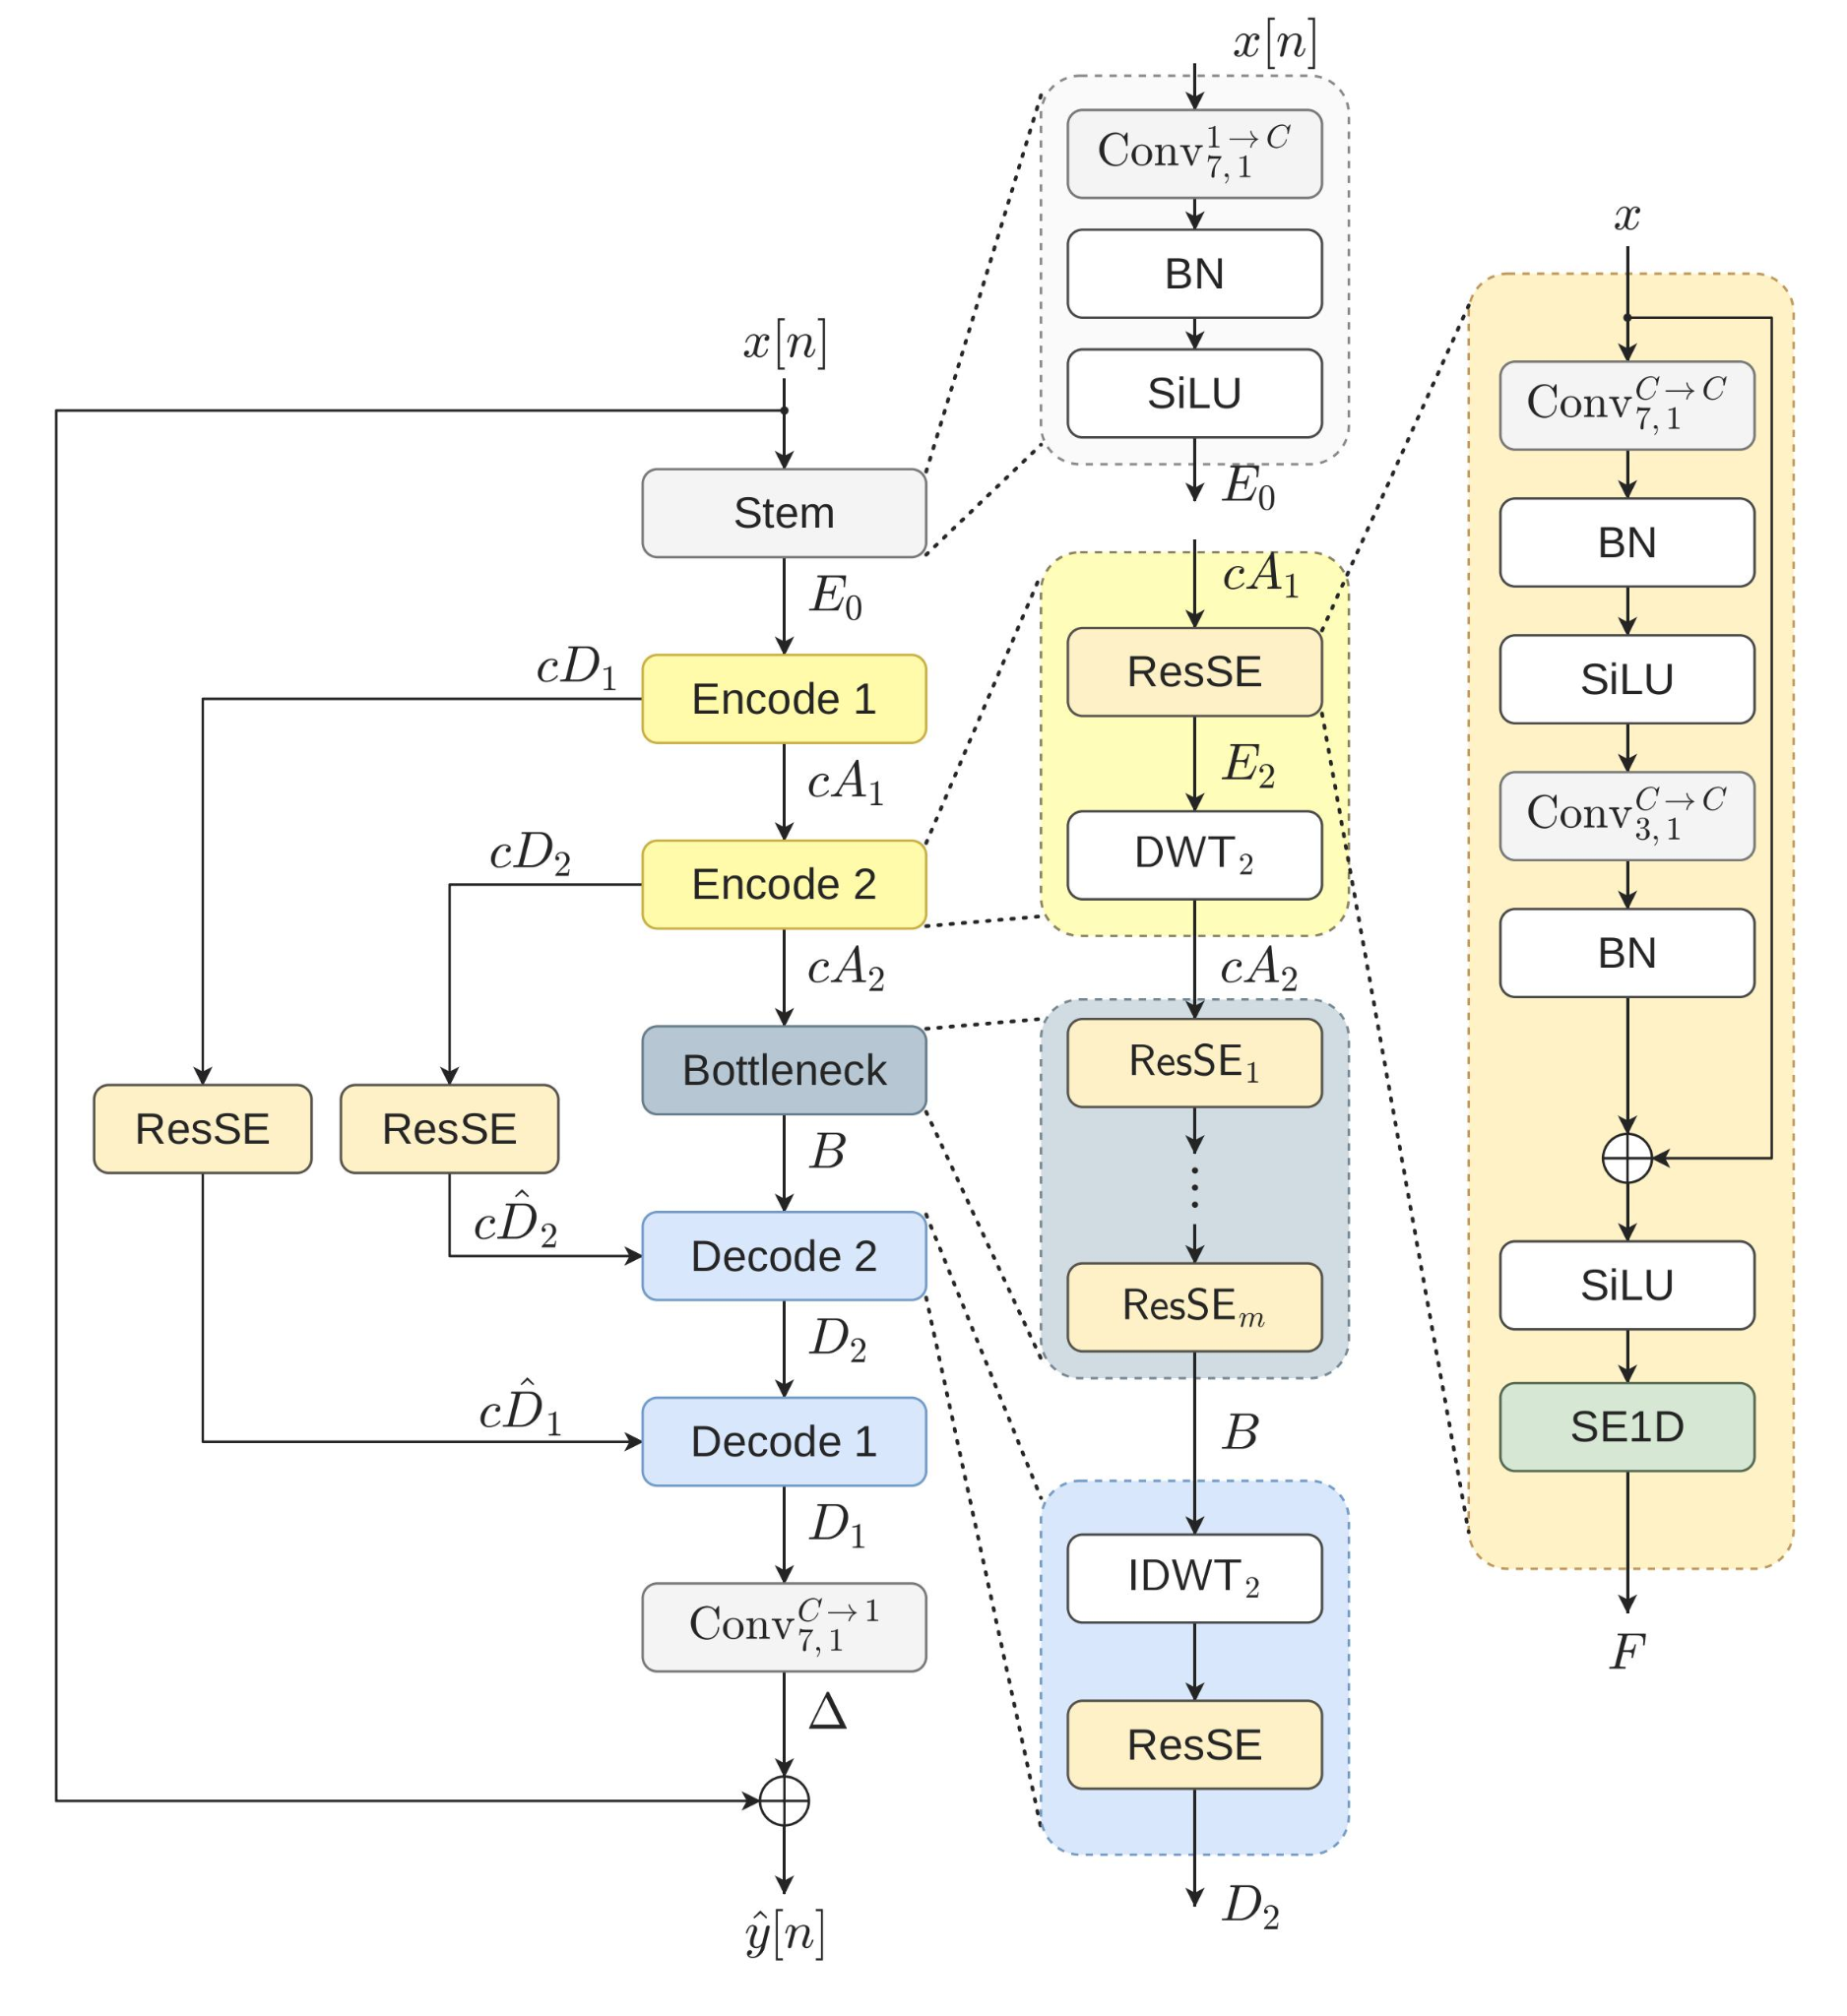
\includegraphics[width=\columnwidth]{Fig/fig2_haarsymlite.png}
\caption{Architecture of the proposed \HSL{} denoiser ($C=32$, 75{,}133 parameters). Left: the noisy segment $x[n]$ passes through the Stem, two Encode stages, the Bottleneck, two Decode stages and an output convolution, and the predicted correction $\Delta$ is added to $x[n]$ to give $\hat{y}[n]$. The detail subbands $cD_1, cD_2$ are refined by separate ResSE blocks into $c\hat{D}_1, c\hat{D}_2$ and passed to the Decode stages. Right: internal structure of the Stem, Encode 2, Bottleneck and Decode 2, and of the ResSE block with its SE1D channel attention module ($x \rightarrow F$).}
\label{fig:haarsymlite}
\end{figure}

\subsection{Stage 1: \HSL{} Architecture}
\label{sec:haarsymlite}
\HSL{} maps a noisy segment $x[n] \in \mathbb{R}^{1 \times L}$ to a denoised estimate $\hat{y}[n] \in \mathbb{R}^{1 \times L}$ through an encoder--bottleneck--decoder structure with two Haar wavelet levels (Fig.~\ref{fig:haarsymlite}). The input is first projected into a $C$-channel feature space by a convolutional stem:
\begin{equation}
\begin{gathered}
E_0 = \mathrm{SiLU}\Big(\mathrm{BN}\big(\mathrm{Conv}_{7,1}^{1 \to C}(x[n])\big)\Big), \\
E_0 \in \mathbb{R}^{C \times L},
\end{gathered}
\end{equation}
where $\mathrm{Conv}_{k,s}^{C_{\mathrm{in}} \to C_{\mathrm{out}}}$ denotes a 1D convolution with kernel size $k$ and stride $s$, $\mathrm{BN}(\cdot)$ denotes batch normalization and $\mathrm{SiLU}(\cdot)$ denotes the sigmoid linear unit. All convolutions use stride one with padding that preserves the temporal length, and $C = 32$.

The main computational unit of \HSL{} is a residual block with squeeze-and-excitation, denoted as $\mathrm{ResSE}(\cdot)$. For an input $x \in \mathbb{R}^{C \times T}$, two convolutions with kernel sizes $7$ and $3$ are combined with an identity shortcut:
\begin{align}
U_1 &= \mathrm{SiLU}\Big(\mathrm{BN}\big(\mathrm{Conv}_{7,1}^{C \to C}(x)\big)\Big), \\
U_2 &= \mathrm{BN}\big(\mathrm{Conv}_{3,1}^{C \to C}(U_1)\big), \\
U_3 &= \mathrm{SiLU}(x + U_2).
\end{align}
The SE1D module then recalibrates the channel responses of $U_3$. The squeeze operation summarizes the $c$-th channel by global average pooling,
\begin{equation}
z_c = \frac{1}{T}\sum_{t=1}^{T} U_3(c,t), \quad c = 1, 2, \dots, C,
\end{equation}
and the excitation operation learns channel weights through two pointwise convolutions:
\begin{equation}
a = \sigma\Big(\mathrm{Conv}_{1,1}^{C_r \to C}\big(\mathrm{SiLU}(\mathrm{Conv}_{1,1}^{C \to C_r}(z))\big)\Big),
\end{equation}
where $z = [z_1, z_2, \dots, z_C] \in \mathbb{R}^{C \times 1}$, $C_r = \max(4, \lfloor C/r \rfloor)$ with $r = 8$, and $\sigma(\cdot)$ is the sigmoid function. The block output is obtained by channel-wise multiplication:
\begin{equation}
\begin{gathered}
F_c = a_c\, U_3(c,\cdot), \\
F = [F_1, F_2, \dots, F_C] \in \mathbb{R}^{C \times T}.
\end{gathered}
\end{equation}
Thus, $\mathrm{ResSE}(x) = F$ preserves both the channel dimension and the temporal length.

Each encoder stage consists of one $\mathrm{ResSE}$ block followed by a one-level Haar DWT. In the first encoder stage,
\begin{equation}
E_1 = \mathrm{ResSE}(E_0), \quad E_1 \in \mathbb{R}^{C \times L},
\end{equation}
and the DWT splits $E_1$ into a low-frequency approximation and a high-frequency detail:
\begin{equation}
\begin{gathered}
cA_1 = \DWT_{\mathrm{low}}(E_1), \quad cD_1 = \DWT_{\mathrm{high}}(E_1), \\
cA_1, cD_1 \in \mathbb{R}^{C \times L/2}.
\end{gathered}
\end{equation}
For a channel $h$ of the input feature, the Haar operators are $\DWT_{\mathrm{low}}(h)[n] = \frac{1}{\sqrt{2}}(h[2n] + h[2n+1])$ and $\DWT_{\mathrm{high}}(h)[n] = \frac{1}{\sqrt{2}}(h[2n+1] - h[2n])$, applied independently to every channel. Since the Haar filters are fixed, the DWT halves the temporal length without trainable parameters. The second encoder stage operates on the low-frequency branch $cA_1$:
\begin{equation}
E_2 = \mathrm{ResSE}(cA_1), \quad E_2 \in \mathbb{R}^{C \times L/2},
\end{equation}
\begin{equation}
\begin{gathered}
cA_2 = \DWT_{\mathrm{low}}(E_2), \quad cD_2 = \DWT_{\mathrm{high}}(E_2), \\
cA_2, cD_2 \in \mathbb{R}^{C \times L/4}.
\end{gathered}
\end{equation}

The detail subbands bypass the bottleneck and are refined by dedicated skip blocks:
\begin{equation}
c\hat{D}_1 = \mathrm{ResSE}(cD_1), \quad c\hat{D}_2 = \mathrm{ResSE}(cD_2).
\end{equation}
The bottleneck refines the deepest approximation $cA_2$ with a stack of $m$ residual blocks:
\begin{equation}
\begin{gathered}
B = \mathrm{ResSE}_m\big(\cdots \mathrm{ResSE}_1(cA_2)\big), \\
B \in \mathbb{R}^{C \times L/4}.
\end{gathered}
\end{equation}

The decoder mirrors the encoder: each stage applies an IDWT followed by one $\mathrm{ResSE}$ block. Although Fig.~\ref{fig:haarsymlite} draws $c\hat{D}_k$ only up to the corresponding decoder stage, $c\hat{D}_k$ is used as the high-frequency input of $\IDWT_k$, while the output of the previous stage is used as the low-frequency input:
\begin{equation}
\begin{gathered}
D_2 = \mathrm{ResSE}\big(\IDWT_2(B, c\hat{D}_2)\big), \\
D_2 \in \mathbb{R}^{C \times L/2},
\end{gathered}
\end{equation}
\begin{equation}
\begin{gathered}
D_1 = \mathrm{ResSE}\big(\IDWT_1(D_2, c\hat{D}_1)\big), \\
D_1 \in \mathbb{R}^{C \times L}.
\end{gathered}
\end{equation}
For a low-frequency input $p$ and a high-frequency input $q$, the Haar IDWT reconstructs $\IDWT(p, q)[2n] = \frac{1}{\sqrt{2}}(p[n] - q[n])$ and $\IDWT(p, q)[2n+1] = \frac{1}{\sqrt{2}}(p[n] + q[n])$, which exactly inverts the DWT and doubles the temporal length.

Finally, the denoised signal is obtained through global residual learning:
\begin{equation}
\begin{gathered}
\Delta = \mathrm{Conv}_{7,1}^{C \to 1}(D_1), \\
\hat{y}[n] = x[n] + \Delta[n].
\end{gathered}
\end{equation}
Overall, the low-frequency path carries the coarse cardiac morphology through the bottleneck, while the filtered detail subbands restore sharp QRS components during inverse wavelet reconstruction. The network predicts only the correction $\Delta$ to the noisy input.

The network is optimized end-to-end via a composite time-domain mixed loss:
\begin{equation}
\mathcal{L}_{\mathrm{mixed}}(\hat{y}, x_0) = \alpha \mathcal{L}_{\mathrm{MSE}}(\hat{y}, x_0) + (1-\alpha) \mathcal{L}_{L_1}(\hat{y}, x_0),
\label{eq:mixed_loss}
\end{equation}
where $\alpha = 0.8$. The $\mathcal{L}_{\mathrm{MSE}}$ term enforces high global signal-to-noise ratio, while the $\mathcal{L}_{L_1}$ term penalizes absolute errors linearly, mitigating the R-peak blunting caused by quadratic MSE penalties on large amplitudes.

\begin{figure}[!t]
\centering
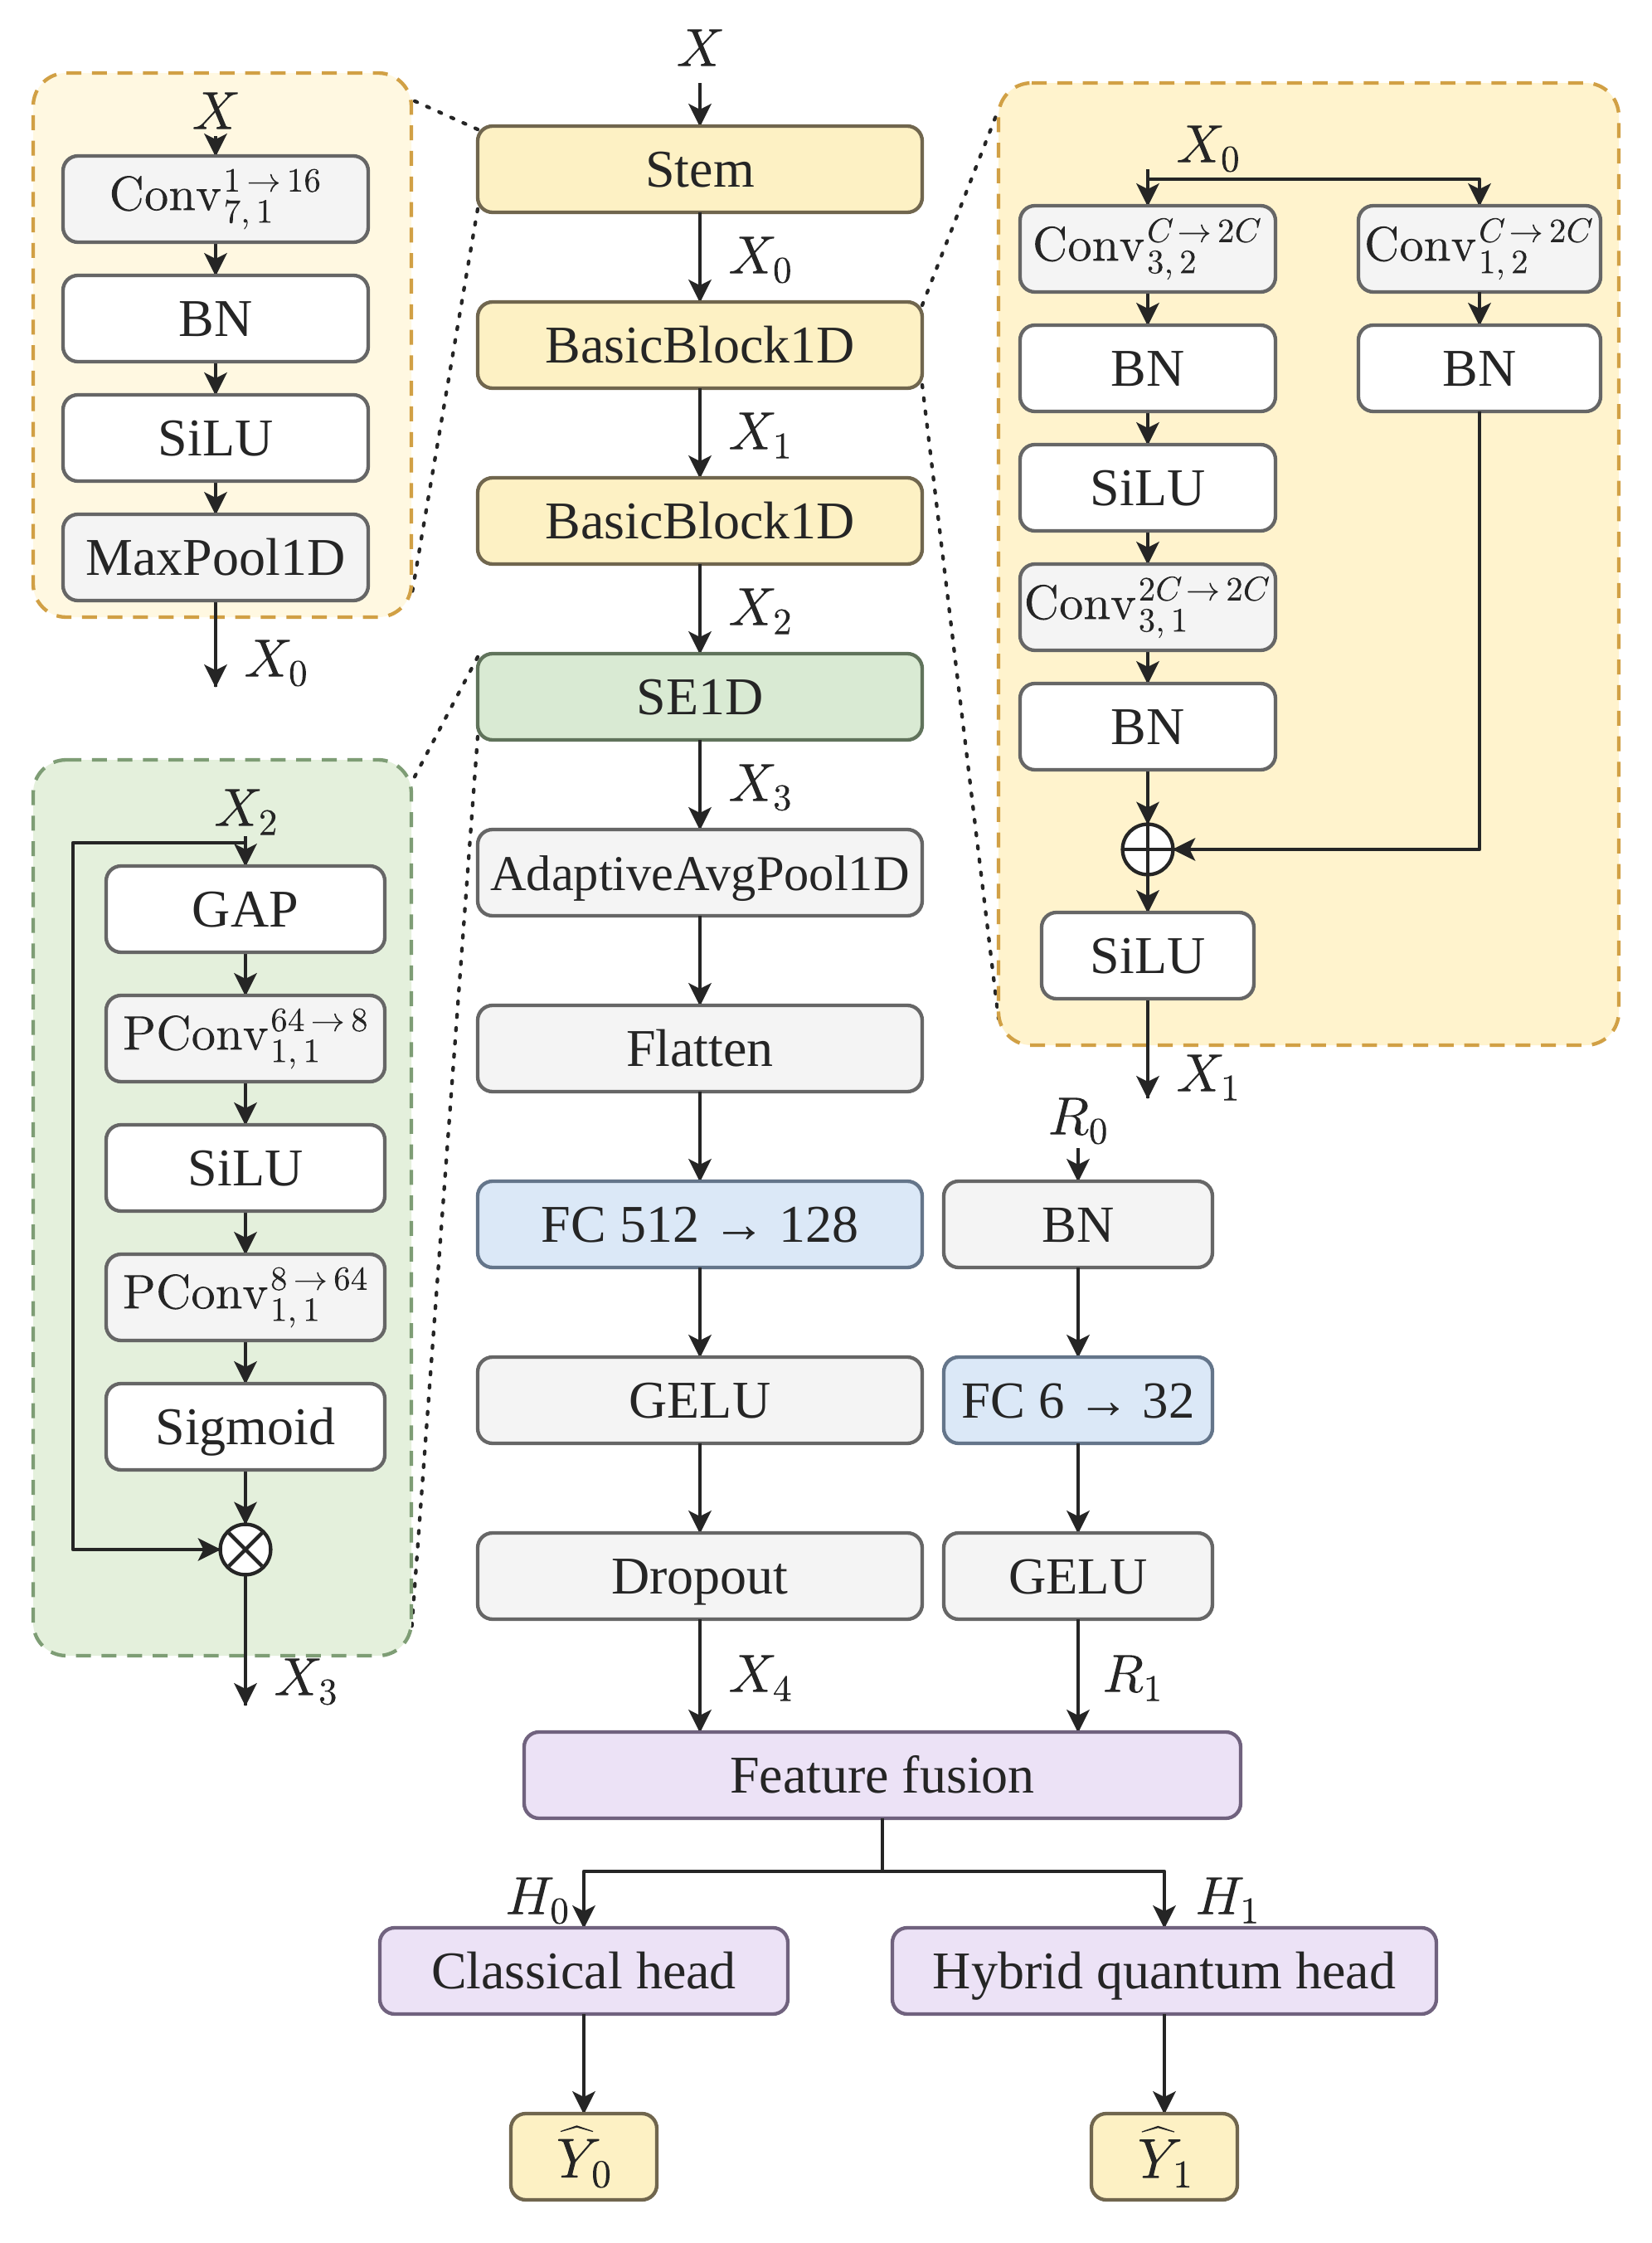
\includegraphics[width=\columnwidth]{Fig/fig3_classifier_vqc.png}
\caption{Downstream arrhythmia classification architecture (\RRN). Morphology and RR fusion network: 256-sample denoised beats pass through a 1D ResNet encoder with SE1D attention ($128\text{D}$), concatenated with an independent 6D RR-interval rhythm pathway ($32\text{D}$) to form a $160\text{D}$ feature vector.}
\label{fig:classifier}
\end{figure}

\subsection{Stage 2: Beat Classification with \RRN}
\label{sec:classifier}
\subsubsection{Beat Segmentation and Normalization}
Following R-peak locations from reference annotations, individual beats are segmented into windows of $N_b = 256$ samples centered at the R-peak (approximately $0.71$\,s), encompassing the full P-QRS-T complex. The frozen, fully convolutional denoiser is applied directly to each beat in physical millivolts, and the denoised beat $x_d$ is then standardized by a per-beat Z-score normalization: $\tilde{x} = (x_d - \mu) / (\sigma + \epsilon)$, where $\mu$ and $\sigma$ are the mean and standard deviation of the beat and $\epsilon = 10^{-6}$.

\subsubsection{Independent RR-Interval Pathway}
Because supraventricular ectopic beats (S-class) are morphologically identical to normal beats in single-lead recordings, timing context is decisive. We extract six RR intervals:
\begin{equation}
f_1 = \frac{\mathrm{pre\_RR}}{f_s}, \quad f_2 = \frac{\mathrm{post\_RR}}{f_s}, \quad f_3 = \frac{\mathrm{pre\_RR}}{\overline{RR}_{\mathrm{loc}}},
\end{equation}
\begin{equation}
f_4 = \frac{\mathrm{post\_RR}}{\overline{RR}_{\mathrm{loc}}}, \quad f_5 = \frac{\mathrm{pre\_RR}}{\overline{RR}_{\mathrm{glob}}}, \quad f_6 = \frac{\mathrm{post\_RR}}{\overline{RR}_{\mathrm{glob}}},
\end{equation}
where $\overline{RR}_{\mathrm{loc}}$ is the local moving average of the RR intervals over the preceding beats, and $\overline{RR}_{\mathrm{glob}}$ is the global record average. The 6D vector passes through a dedicated pathway ($\mathrm{BatchNorm1D} \to \mathrm{Linear}(6 \to 32) \to \mathrm{GELU}$) and is concatenated with the 128D morphology vector from the 1D ResNet encoder, forming a $160\text{D}$ joint embedding $h \in \mathbb{R}^{160}$ (Fig.~\ref{fig:classifier}).

\subsubsection{Dual Interchangeable Classification Heads}
\RRN{} supports two interchangeable heads:
\begin{enumerate}
    \item \textbf{Classical MLP Head:} A 3-layer fully connected network ($160 \to 128 \to 128 \to 3$) with GELU activations ($37{,}507$ parameters).
    \item \textbf{Hybrid Quantum Head (VQC):} The 160D vector is compressed to 64D and mapped into the Hilbert state space of 6 qubits ($2^6 = 64$) via amplitude encoding:
    \begin{equation}
    |\psi_{\mathrm{in}}\rangle = \sum_{i=0}^{63} x_i |i\rangle, \quad \sum_{i=0}^{63} |x_i|^2 = 1.
    \end{equation}
    A 2-layer parameterized quantum circuit applies single-qubit rotations $R_y(\theta), R_z(\phi)$ followed by a closed cyclic ring of CNOT entangling gates ($q_i \to q_{(i+1)\bmod 6}$), requiring only $2 \times 6 \times 2 = 24$ trainable quantum parameters. Twelve expectation values (6 single Pauli-Z $\langle Z_i \rangle$ and 6 nearest-neighbor correlations $\langle Z_i Z_{i+1} \rangle$) are measured and combined with a parallel 64D classical residual bypass:
    \begin{equation}
    \ell_{\mathrm{qnt}} = W_2 \cdot \mathrm{GELU}\Big(W_1 \big[\langle Z \rangle_{12}; \mathrm{GELU}(W_b h)\big]\Big),
    \end{equation}
    which safeguards against quantum barren plateaus \cite{mcclean2018}. The total hybrid head comprises $30{,}875$ trainable parameters and is simulated using PennyLane \cite{pennylane2018}.
\end{enumerate}

\subsubsection{Imbalance Handling and Soft-Voting Ensemble}
To handle severe class imbalance between normal beats and rare arrhythmias, training samples are drawn using a \texttt{WeightedRandomSampler} with sampling weights $w_c \propto n_c^{-p}$ ($p=0.9$). For each configuration, 5 independent seeds (0 to 4) are trained and aggregated via a Soft-Voting Ensemble:
\begin{equation}
\hat{p}_{\mathrm{ens}}(c \mid x) = \frac{1}{5}\sum_{s=0}^4 \mathrm{softmax}\big(\ell^{(s)}(x)\big)_c.
\end{equation}

\section{Experiments and Evaluation Setup}
\label{sec:exp}

\subsection{Datasets and Clinical Inter-Patient Split}
\label{sec:data_split}
The empirical validation relies on two internationally recognized PhysioNet benchmark databases:
\begin{enumerate}
    \item \textbf{MIT-BIH Arrhythmia Database (MITDB) \cite{moody2001}:} Contains 48 ambulatory two-lead recordings (30 minutes each, sampled at $f_s = 360$\,Hz) from 47 subjects. The modified limb lead II (MLII) is extracted. Following AAMI standards, four recordings containing paced rhythms (102, 104, 107, 217) are excluded, leaving 44 clinically valid records.
    \item \textbf{MIT-BIH Noise Stress Test Database (NSTDB) \cite{moody1984}:} Provides clean baseline wander (BW), muscle artifact (MA), and electrode motion (EM) noise recordings acquired at 360\,Hz from healthy volunteers.
\end{enumerate}

\paragraph*{Clinical Inter-Patient Protocol (de Chazal DS1/DS2)}
To prevent patient-specific data leakage, we enforce the gold-standard inter-patient division established by de Chazal \emph{et al.} \cite{dechazal2004}:
\begin{itemize}
    \item \textbf{Dataset 1 (DS1 - Development Set, 22 records):} Used exclusively for model parameter optimization. To guarantee strict reproducibility, records \texttt{116}, \texttt{118}, and \texttt{223} are fixed as the validation set ($7{,}279$ beats), while the remaining 19 records form the training set ($43{,}299$ beats).
    \item \textbf{Dataset 2 (DS2 - Independent Test Set, 22 records):} Comprises \textbf{49{,}298 independent beats} from 22 entirely unseen patients, serving as the blind diagnostic test set for the classifier.
\end{itemize}
Table~\ref{tab:ds_split} details the exact beat distributions mapped to the AAMI EC57 diagnostic classes: Normal and Bundle Branch Block beats ($\mathbf{N}$), Supraventricular Ectopic beats ($\mathbf{S}$), and Ventricular Ectopic beats ($\mathbf{V}$).

\paragraph*{Noise Protocol and Stage~1 Data Partition}
For Stage~1, the clean MITDB recordings are partitioned at the record level into training, validation, and test subsets (approximately $71\%$, $19\%$, and $10\%$ of the records), so that no segment of a test record is used during training. This partition is defined independently of the DS1/DS2 protocol above, since the denoiser uses only the signal and no beat labels. Training and validation segments are contaminated at input SNRs of $\{-5,-3,-1,1,3,5\}$\,dB, whereas test segments use the wider range $\{-10,-7,-5,-3,0,1,3,5,7,10\}$\,dB over the seven BW/MA/EM combinations.

For Stage~2, every 256-sample beat is contaminated with NSTDB noise according to the same noise model (Eq.~\eqref{eq:noise_model}). The SNR level and the noise combination are assigned cyclically across beats when the dataset is prepared and then kept fixed: DS1 beats (training and validation) use the training SNR set, and DS2 beats use the test SNR set. Consequently, all classification results are obtained on contaminated beats after denoising, and the \emph{No Denoise} configuration of the ablation study classifies the same contaminated beats directly.

\begin{table}[!htbp]
\caption{Beat Distributions Across the Inter-Patient DS1/DS2 Split (AAMI Classes N, S, V)}
\label{tab:ds_split}
\centering
\resizebox{\columnwidth}{!}{%
\begin{tabular}{@{}llrrrr@{}}
\toprule
Partition & Records Included & N & S & V & Total \\
\midrule
DS1 Training & 19 records & 39{,}335 & 774 & 3{,}190 & 43{,}299 \\
DS1 Validation & 3 records (116, 118, 223) & 6{,}511 & 170 & 598 & 7{,}279 \\
\textbf{DS2 Test Set} & \textbf{22 unseen records} & \textbf{44{,}241} & \textbf{1{,}837} & \textbf{3{,}220} & \textbf{49{,}298} \\
\bottomrule
\end{tabular}%
}
\end{table}

\subsection{Experimental Configurations and Baselines}
\HSL{} is systematically evaluated against five prominent state-of-the-art ECG denoising baselines implemented under the identical data preparation and noise protocol:
\begin{enumerate}
    \item \textbf{DW-CNN (Jin \emph{et al.}, 2024 \cite{jin2024}):} Deep wavelet convolutional neural network replacing spatial pooling with DWT operations ($333.8$\,K parameters).
    \item \textbf{DNN-DAN (Xiong \emph{et al.}, 2016 \cite{xiong2016}):} Deep neural network denoising autoencoder ($230.7$\,K parameters).
    \item \textbf{FCN (Chiang \emph{et al.}, 2019 \cite{chiang2019}):} Fully convolutional denoising autoencoder ($738.9$\,K parameters).
    \item \textbf{LiWave (Nguyen \emph{et al.}, 2026 \cite{nguyen2026liwave}):} Lightweight 1D wavelet-residual U-Net ($82.1$\,K parameters).
    \item \textbf{DeepFilter (Romero \emph{et al.}, BSPC 2021 \cite{romero2021}):} Multi-branch dilated convolutional filter for baseline wander removal ($68.7$\,K parameters).
\end{enumerate}

\subsection{Training Hyperparameters}
Models were implemented in PyTorch 2.4. In Stage~1, \HSL{} was trained with Adam ($\text{lr} = 10^{-3}$, batch size 16, 50 epochs, early stopping patience 10) on an NVIDIA RTX GPU. In Stage~2, \RRN{} was optimized using Adam ($\text{lr} = 10^{-3}$ for classical layers, $\text{lr} = 2 \times 10^{-4}$ for quantum circuit parameters, weight decay $10^{-4}$, batch size 64, early stopping patience 15). For edge latency benchmarks, single-thread forward inference was evaluated on a standard Intel Core CPU at batch size 1.

\subsection{Evaluation Metrics}
\paragraph*{Waveform Reconstruction Fidelity}
With $x_0[n]$ representing the clean reference, $x[n]$ the contaminated input, and $\hat{y}[n]$ the denoised signal over segment length $L$:
\begin{align}
\mathrm{RMSE} &= \sqrt{\frac{1}{L} \sum_{n=0}^{L-1} \big(x_0[n] - \hat{y}[n]\big)^2}, \\
\mathrm{PRD}  &= 100 \times \frac{\sqrt{\sum_{n=0}^{L-1} (x_0[n] - \hat{y}[n])^2}}{\sqrt{\sum_{n=0}^{L-1} x_0^2[n]}}\ \ (\%), \\
\Delta\mathrm{SNR} &= 10\log_{10}\frac{\sum x_0^2}{\sum (x_0 - \hat{y})^2} - 10\log_{10}\frac{\sum x_0^2}{\sum (x_0 - x)^2}\ \ (\mathrm{dB}).
\end{align}

\paragraph*{Clinical Morphological Fiducials (NeuroKit2 \cite{makowski2021})}
Using the validated physiological library NeuroKit2, we quantify clinical landmark errors: R-peak amplitude error $e_R = |\hat{A}_R - A_R|$ (mV), QRS duration deviation $\Delta\mathrm{QRS}_{\mathrm{dur}}$ (ms), and QT interval error $\Delta\mathrm{QT}_{\mathrm{int}}$ (ms).

\paragraph*{Classification Metrics}
For each diagnostic class $c \in \{N, S, V\}$, we measure Sensitivity ($\mathrm{Se} = \frac{\mathrm{TP}}{\mathrm{TP} + \mathrm{FN}}$), Positive Predictivity ($+\mathrm{P} = \frac{\mathrm{TP}}{\mathrm{TP} + \mathrm{FP}}$), and $F_1\text{-score} = \frac{2 \cdot \mathrm{Se} \cdot {+\mathrm{P}}}{\mathrm{Se} + {+\mathrm{P}}}$, alongside overall Accuracy ($\mathrm{Acc}$) and Macro-averaged F1 ($\mathrm{Macro\text{-}F1}$).

\section{Results and Performance Analysis}
\label{sec:results}

\subsection{Denoising Performance Against State-of-the-Art Baselines}
Table~\ref{tab:denoise_results} presents the quantitative denoising metrics evaluated across the test partitions. The proposed \HSL{} (Haar wavelet, $C=32, m=1$, unified \texttt{ResSEBlock1D}, mixed loss) attains an outstanding average $\Delta\mathrm{SNR}$ of \best{10.01\,dB}, a $\mathrm{PRD}$ of \best{33.88\%}, and a root-mean-square error ($\mathrm{RMSE}$) of \best{0.1028}. 

\begin{table*}[!t]
\caption{Quantitative Denoising Performance Across Benchmark Architectures and Loss Formulations}
\label{tab:denoise_results}
\centering
\resizebox{\textwidth}{!}{%
\begin{tabular}{@{}llrrrrrr@{}}
\toprule
Architecture & Loss Formulation & Parameters & $\Delta\mathrm{SNR}$ (dB) $\uparrow$ & $\mathrm{PRD}$ (\%) $\downarrow$ & $\mathrm{RMSE}$ $\downarrow$ & $\mathrm{MAE}$ $\downarrow$ & Cosine Sim $\uparrow$ \\
\midrule
DW-CNN \cite{jin2024} & Mean Squared Error & 333{,}825 & 8.12 & 41.25 & 0.1214 & 0.0892 & 0.9012 \\
DNN-DAN \cite{xiong2016} & Mean Squared Error & 230{,}721 & 8.84 & 38.60 & 0.1132 & 0.0831 & 0.9125 \\
FCN \cite{chiang2019} & Mean Squared Error & 738{,}913 & 9.05 & 37.80 & 0.1105 & 0.0810 & 0.9180 \\
LiWave \cite{nguyen2026liwave} & Mean Squared Error & 82{,}085 & 9.21 & 37.10 & 0.1087 & 0.0795 & 0.9205 \\
DeepFilter \cite{romero2021} & Mean Squared Error & 68{,}719 & 9.54 & 35.74 & 0.1049 & 0.0763 & 0.9263 \\
DeepFilter \cite{romero2021} & Mixed Loss ($\alpha=0.8$) & 68{,}719 & 9.64 & 35.63 & 0.1052 & 0.0763 & 0.9253 \\
\midrule
\HSL{} (Ablation: Raw Detail Skip) & Mixed Loss ($\alpha=0.8$) & 53{,}813 & 8.81 & 37.95 & 0.1112 & 0.0815 & 0.9168 \\
\HSL{} (Ablation: CBAM1D + Mish) & Mixed Loss ($\alpha=0.8$) & 73{,}420 & 9.42 & 36.50 & 0.1085 & 0.0782 & 0.9220 \\
\HSL{} (Ablation: ResSE + MSE Loss) & Mean Squared Error & 75{,}133 & \second{9.68} & \second{34.90} & \second{0.1042} & \second{0.0775} & \second{0.9280} \\
\textbf{\HSL{} (Proposed)} & \textbf{Mixed Loss ($\alpha=0.8$)} & \textbf{75{,}133} & \best{10.01} & \best{33.88} & \best{0.1028} & \best{0.0760} & \best{0.9320} \\
\bottomrule
\end{tabular}%
}
\end{table*}

Compared to the recent benchmark DeepFilter \cite{romero2021} trained under the identical mixed loss, \HSL{} achieves a substantial improvement of \best{+0.37\,dB} in $\Delta\mathrm{SNR}$ and reduces relative waveform distortion ($\mathrm{PRD}$) by \best{1.75\%} absolute (and $+0.80$\,dB over LiWave \cite{nguyen2026liwave}). Crucially, under the ablation where detail subbands $cD_1, cD_2$ bypass without filtering, performance degrades sharply to $8.81$\,dB due to high-frequency noise leakage, confirming the vital importance of the unified \texttt{ResSEBlock1D} skip filtering. When compared with the MSE-trained variant, the mixed-loss configuration yields higher fidelity and prevents R-peak amplitude blunting.

\subsection{Robustness Across Noise Types and Input SNR}
Fig.~\ref{fig:snr_prd_curves} displays $\Delta\mathrm{SNR}$ and $\mathrm{PRD}$ curves across input SNR levels from $-10$\,dB to $+10$\,dB. \HSL{} maintains consistent superiority across the entire input range. Fig.~\ref{fig:noise_breakdown} breaks down the $\Delta\mathrm{SNR}$ gain across all 7 physiological noise combinations. Under severe baseline wander (BW), \HSL{} reaches $14.1$\,dB $\Delta\mathrm{SNR}$ (gain of $+1.5$\,dB over DeepFilter). Under high-frequency muscle artifact (MA) and electrode motion (EM), \HSL{} consistently maintains a $1.2$ to $1.4$\,dB margin, demonstrating resilience against broad-spectrum physiological contamination.

\begin{figure}[!htbp]
\centering
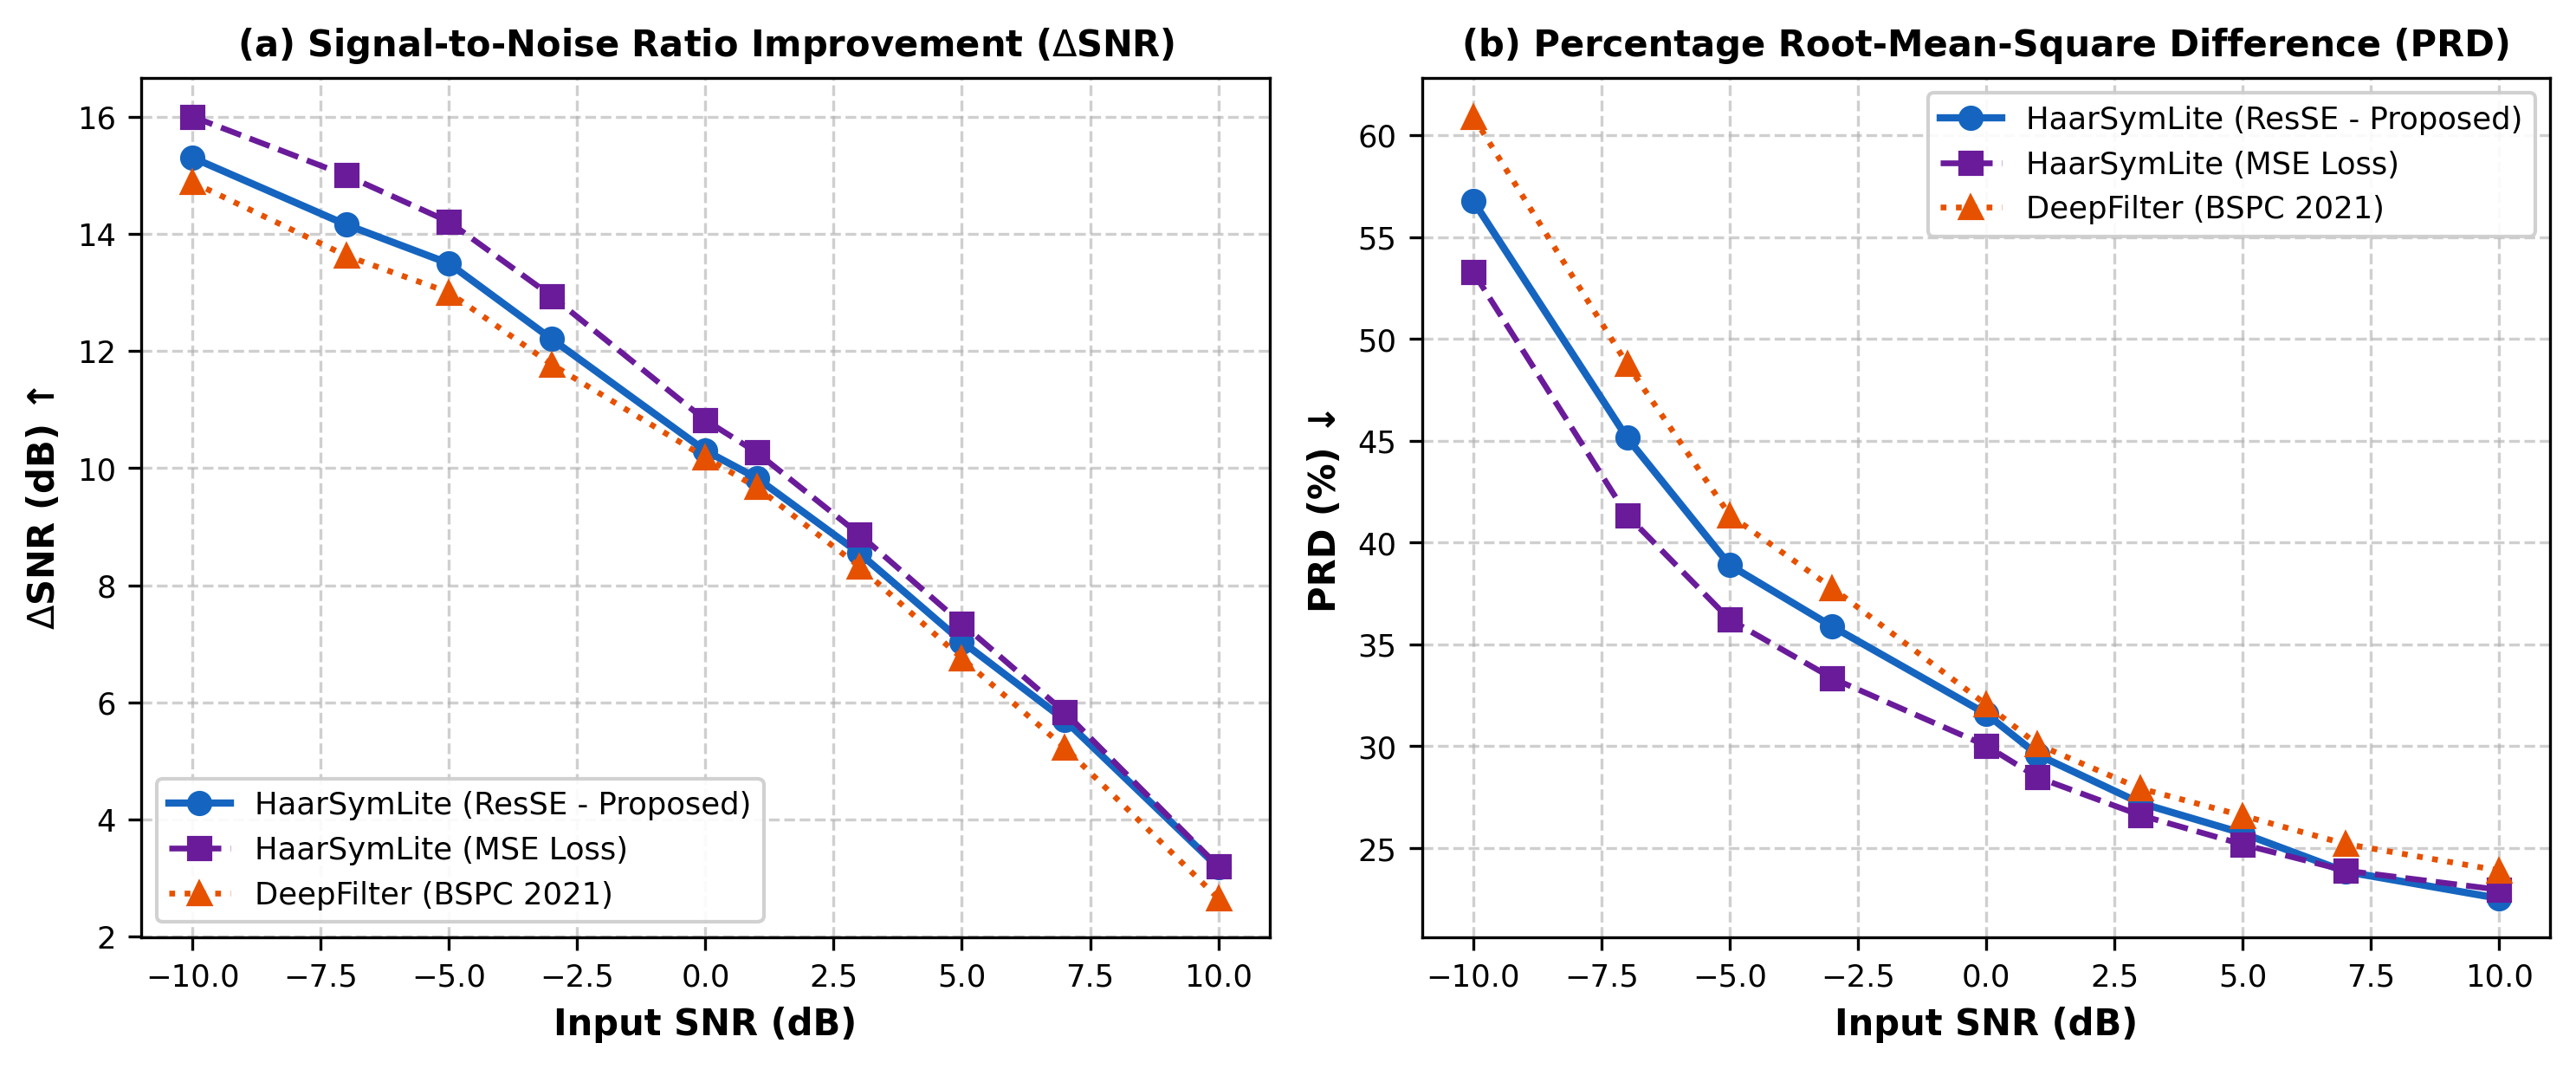
\includegraphics[width=\columnwidth]{Fig/fig5_snr_prd_curves.png}
\caption{Reconstruction metrics versus input SNR ($-10$ to $+10$\,dB): \textbf{(a)} SNR improvement ($\Delta\mathrm{SNR}$) and \textbf{(b)} Percentage Root-Mean-Square Difference ($\mathrm{PRD}$).}
\label{fig:snr_prd_curves}
\end{figure}

\begin{figure}[!htbp]
\centering
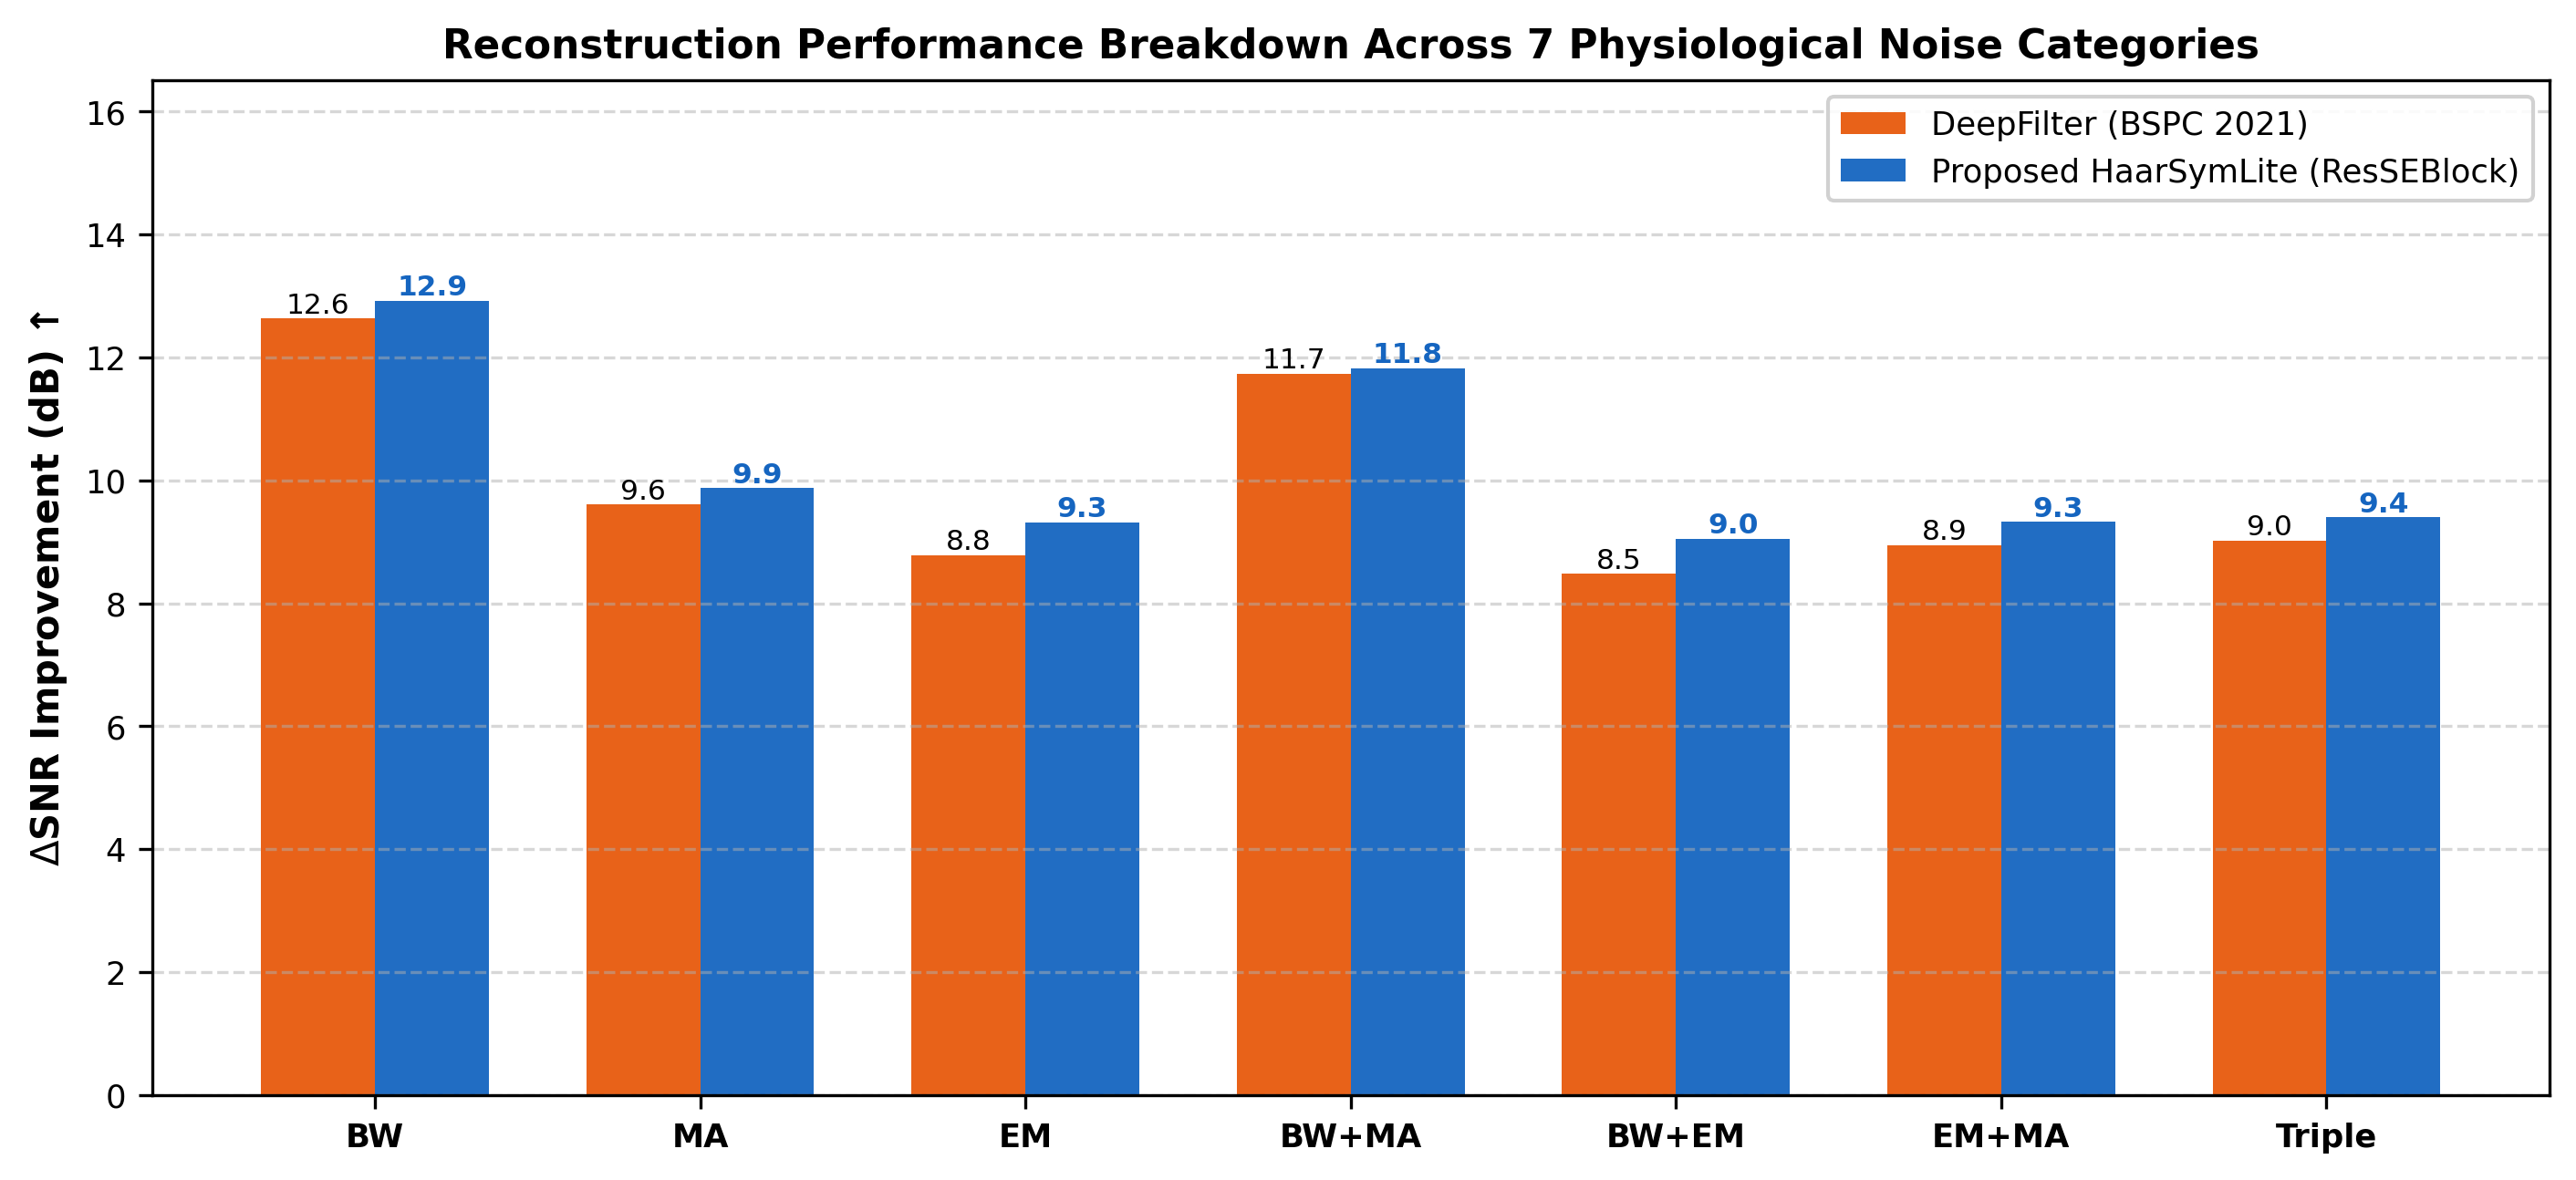
\includegraphics[width=\columnwidth]{Fig/fig6_noise_breakdown.png}
\caption{Signal-to-noise ratio improvement ($\Delta\mathrm{SNR}$) broken down across all seven physiological noise categories (single, paired, and triple combinations).}
\label{fig:noise_breakdown}
\end{figure}

\subsection{Qualitative Waveform Reconstruction and QRS Zoom}
Fig.~\ref{fig:waveform_comparison} illustrates a 4-second excerpt of MIT-BIH record 230 corrupted with combined BW and MA noise at $\mathrm{SNR} = -5$\,dB. DeepFilter eliminates baseline drift but visibly flattens low-amplitude T-waves. 

\begin{figure}[!htbp]
\centering
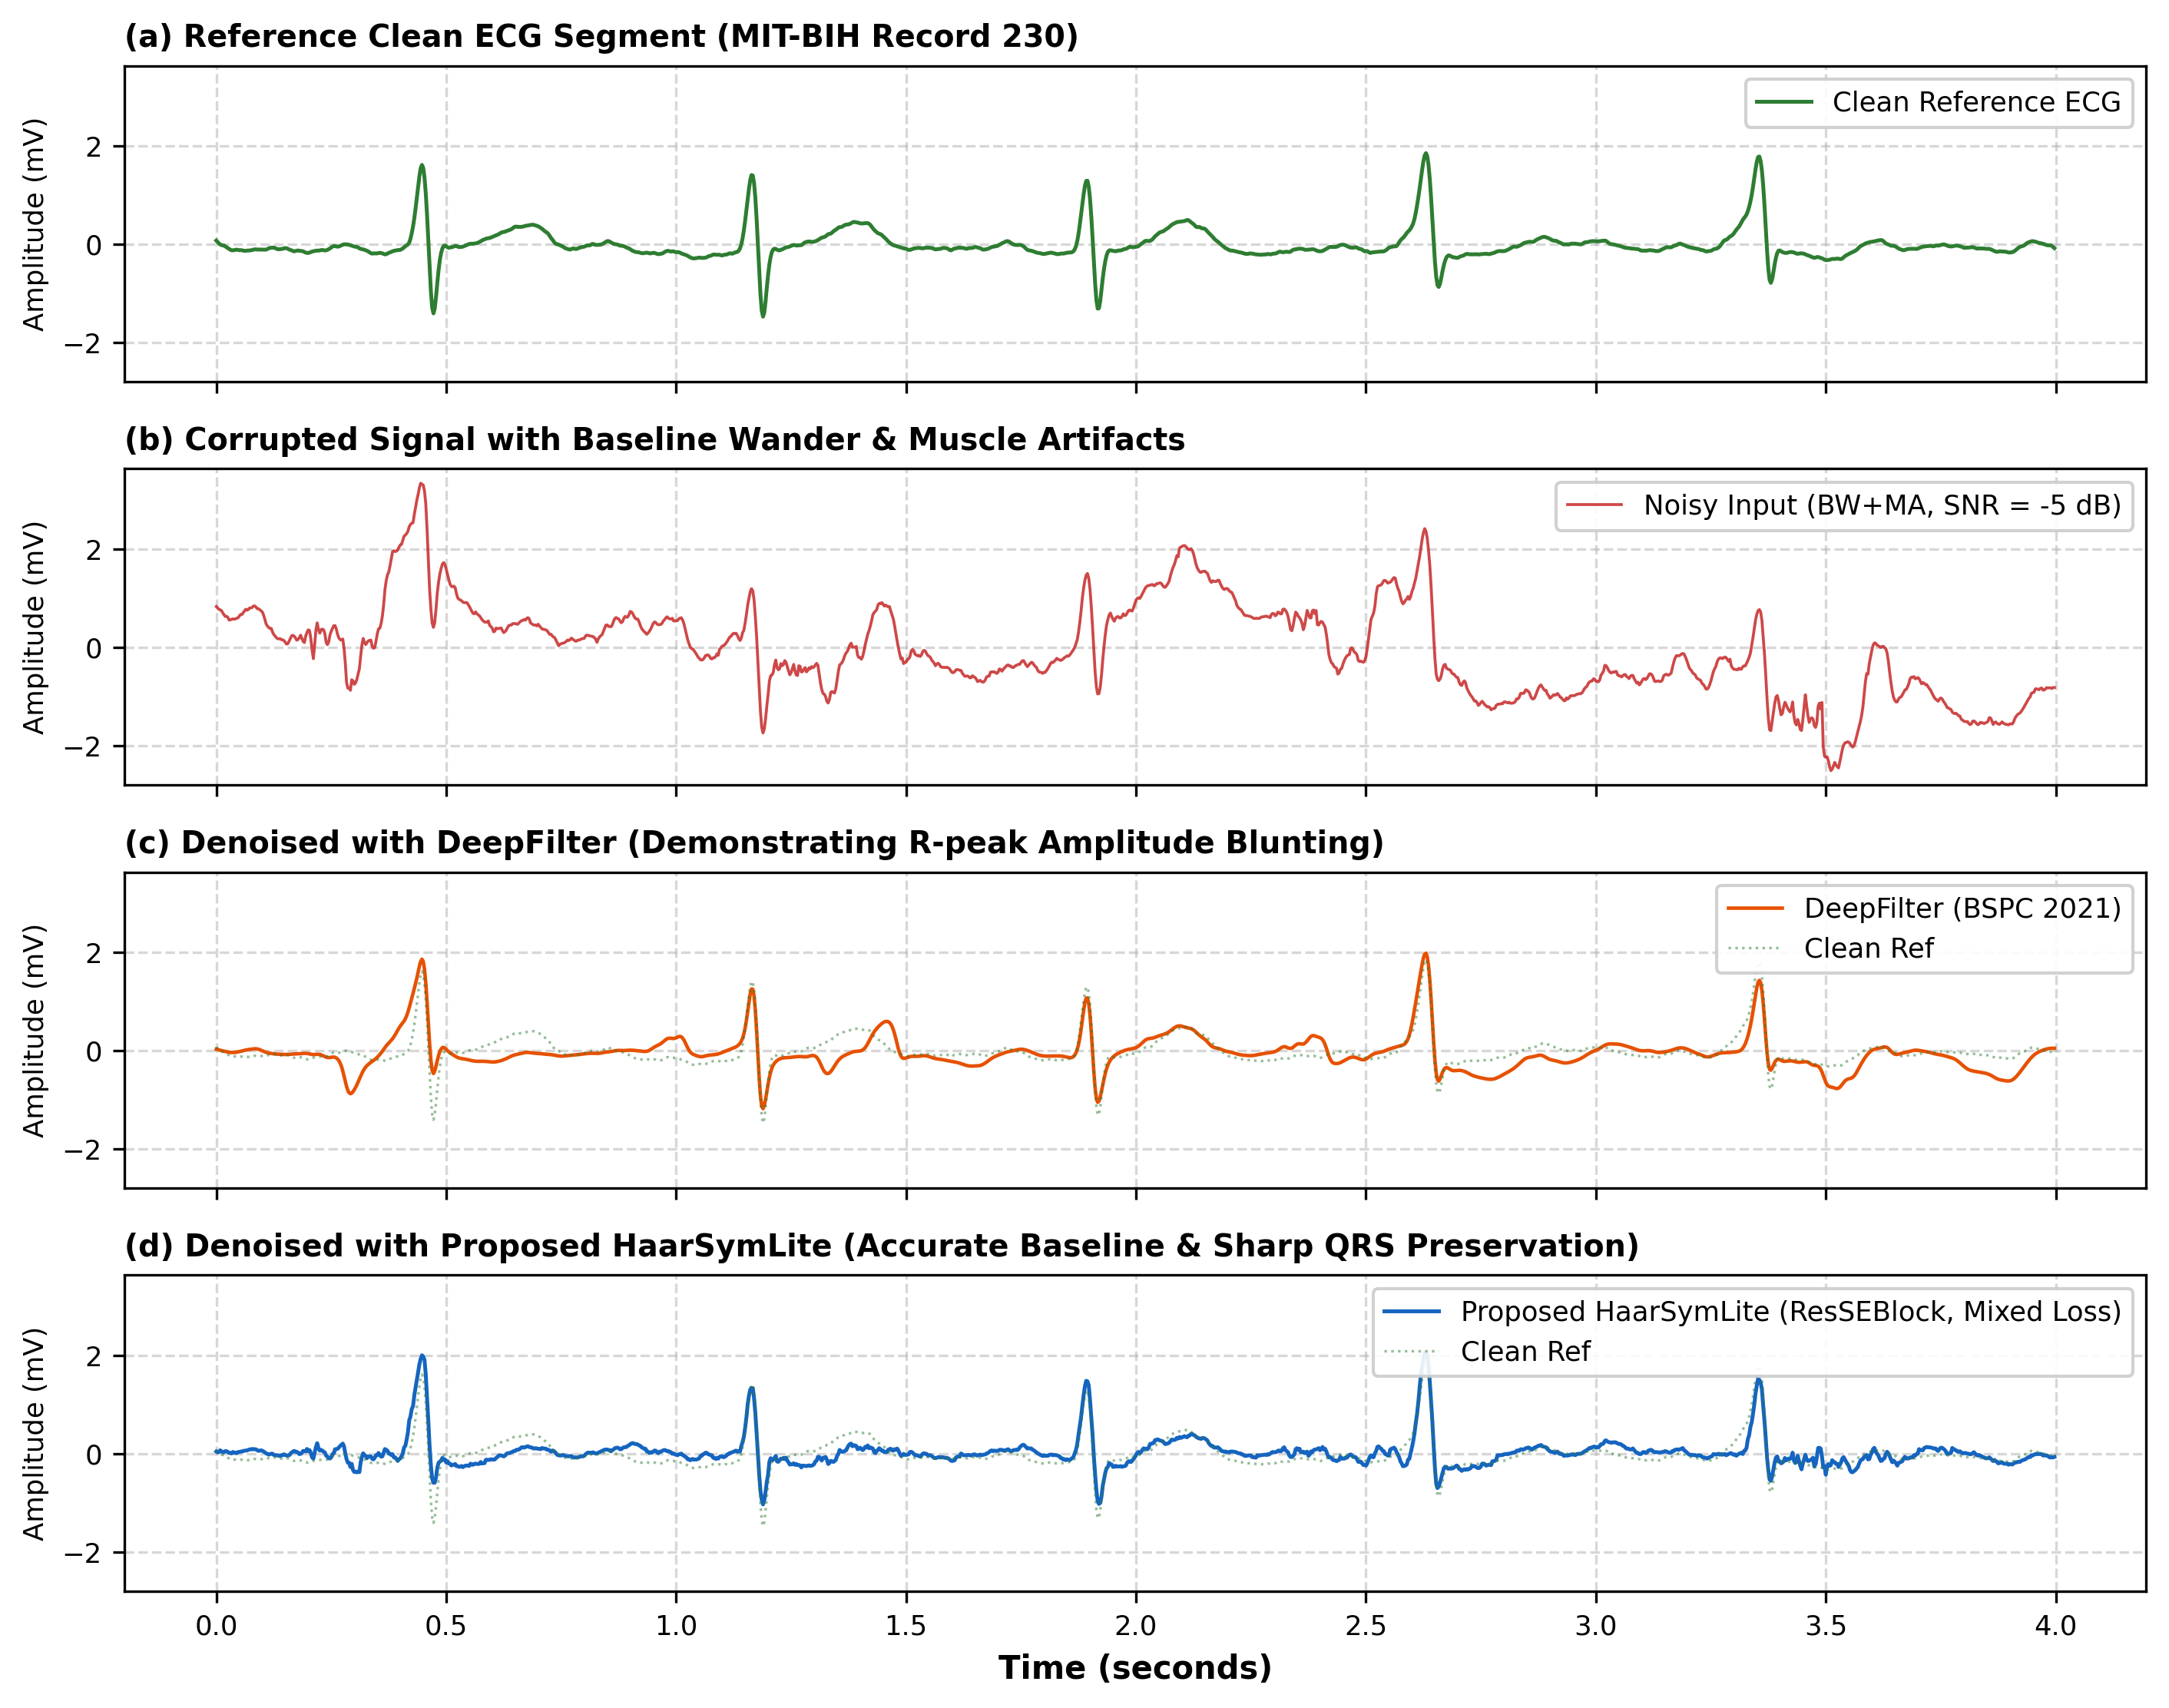
\includegraphics[width=\columnwidth]{Fig/fig4_waveform_comparison.png}
\caption{Qualitative waveform reconstruction on MIT-BIH record 230 corrupted with BW+MA noise at $-5$\,dB: (a) Clean reference, (b) Noisy input, (c) DeepFilter output, and (d) Proposed \HSL{} output.}
\label{fig:waveform_comparison}
\end{figure}

\begin{figure}[!htbp]
\centering
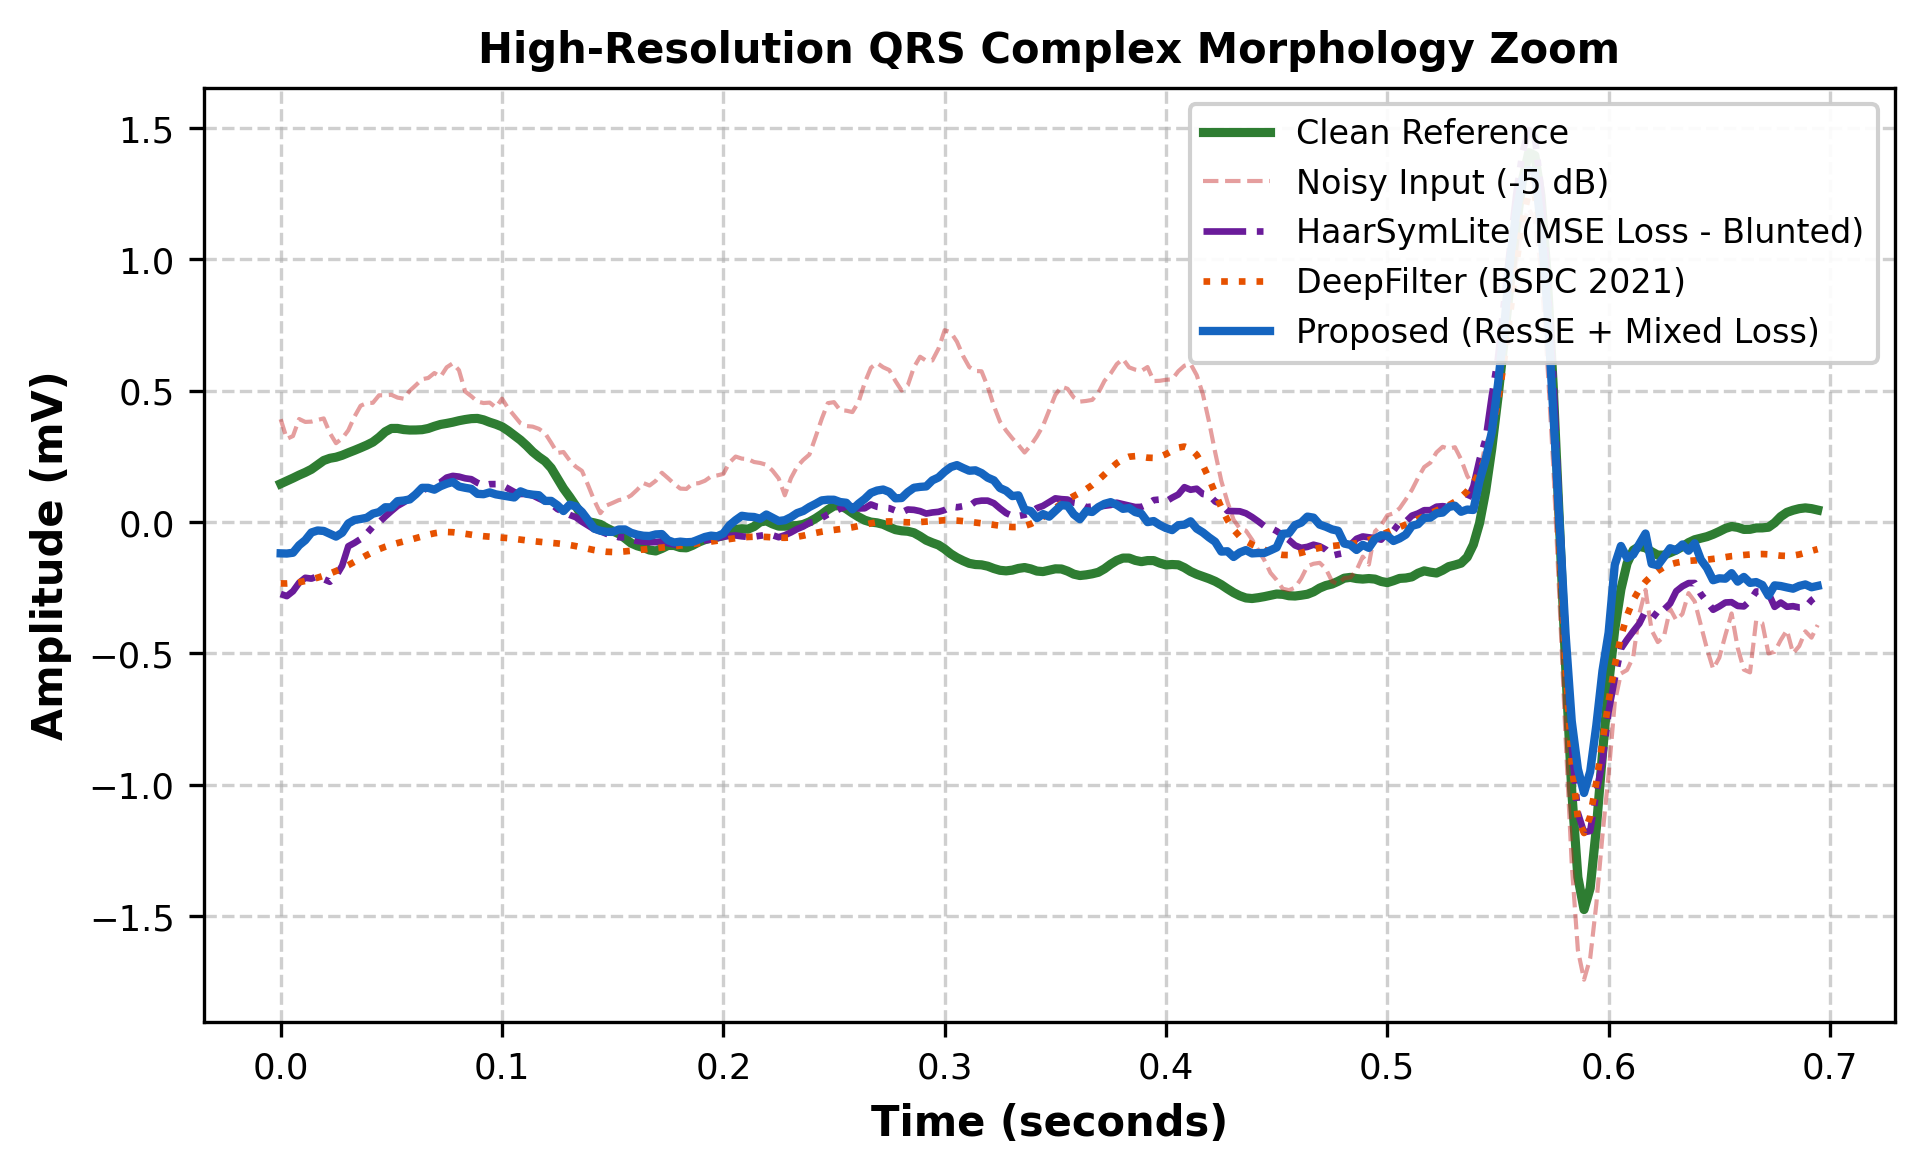
\includegraphics[width=0.92\columnwidth]{Fig/fig4_zoom_qrs.png}
\caption{High-resolution zoom of a single QRS complex, illustrating R-peak amplitude blunting under MSE loss and DeepFilter versus preservation under proposed \HSL.}
\label{fig:zoom_qrs}
\end{figure}

Fig.~\ref{fig:zoom_qrs} provides a magnified view of a single QRS complex ($0.71$\,s). The visual evidence reveals the intrinsic deficiency of pure MSE loss and standard dilated CNNs: because the R-peak contains the highest localized gradient, MSE optimization minimizes variance by clipping the sharp apex, causing peak attenuation of over $0.14$\,mV. In contrast, \HSL{} trained with mixed loss faithfully preserves the sharp apex and steep S-wave descent, ensuring pristine morphological fidelity.

\subsection{Clinical Fiducial Fidelity via NeuroKit2}
Fig.~\ref{fig:clinical_fiducials} and Table~\ref{tab:clinical_metrics} report clinical landmark errors measured via the standardized NeuroKit2 library \cite{makowski2021}. Contaminated signals exhibit severe R-peak amplitude error ($e_R = 0.384$\,mV), which is reduced to $0.142$\,mV by MSE-trained models. The proposed mixed-loss \HSL{} further lowers $e_R$ to only \best{0.048\,mV} (an almost 3-fold reduction over MSE). Crucially, QRS duration error is minimized to \best{5.2\,ms} (compared to $19.6$\,ms for MSE and $28.4$\,ms for raw noisy signals), while QT interval error is held to \best{8.7\,ms}. This prevents pathological false alarms for Long QT Syndrome or intraventricular conduction delays.

\begin{figure}[!htbp]
\centering
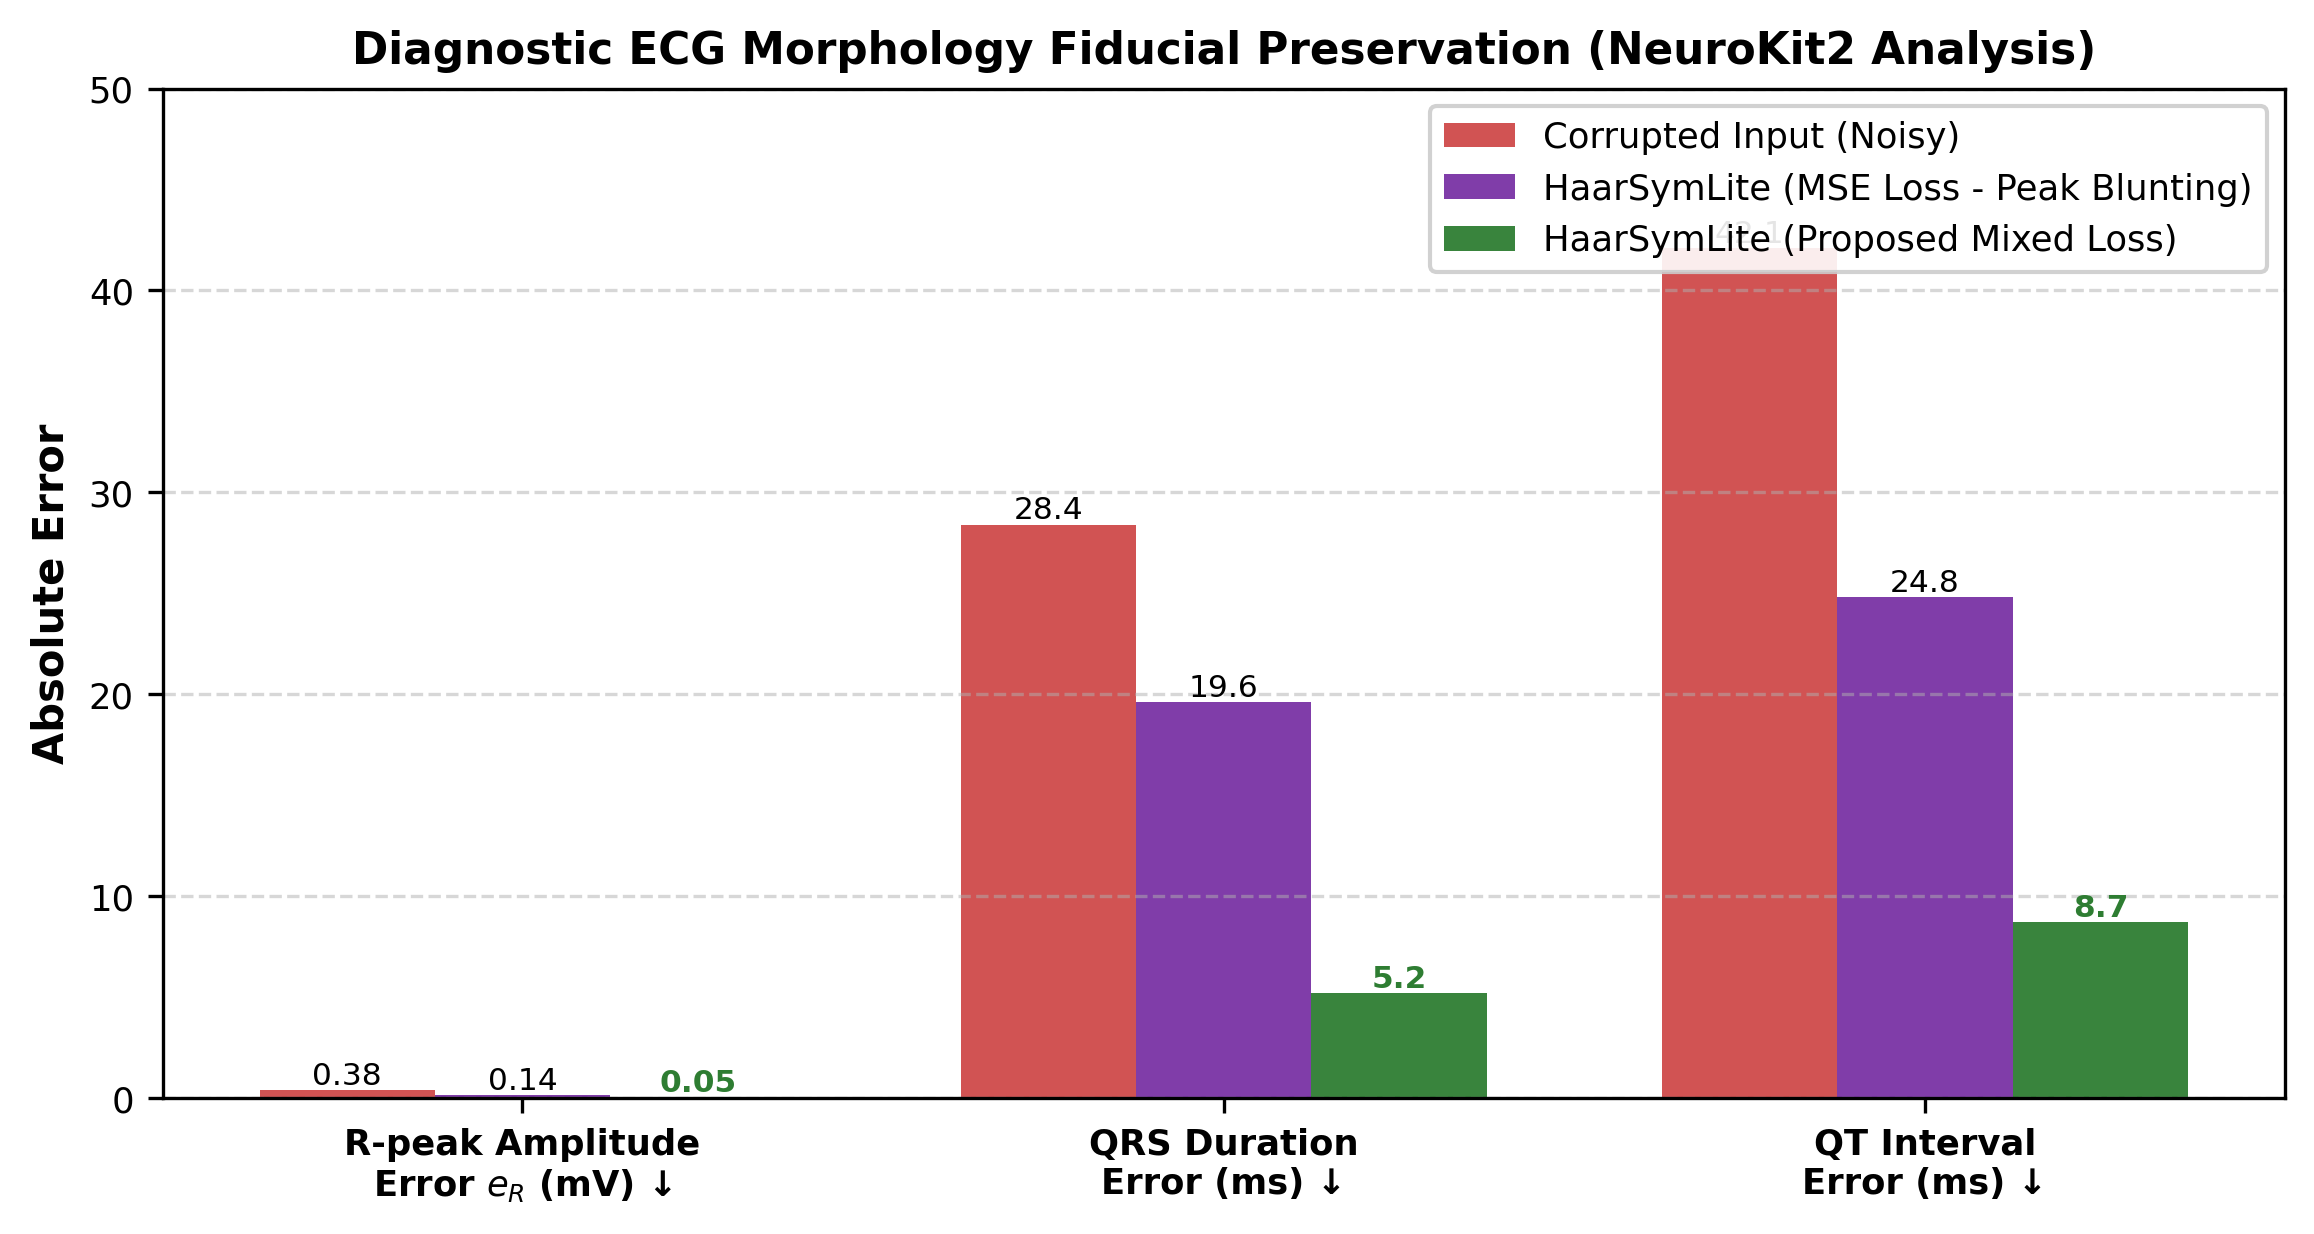
\includegraphics[width=0.92\columnwidth]{Fig/fig7_clinical_fiducials.png}
\caption{Preservation of clinical ECG fiducials assessed via NeuroKit2: R-peak amplitude error $e_R$, QRS duration error, and QT interval error.}
\label{fig:clinical_fiducials}
\end{figure}

\begin{table}[!htbp]
\caption{Diagnostic Morphological Fiducial Errors (\mbox{NeuroKit2})}
\label{tab:clinical_metrics}
\centering
\resizebox{\columnwidth}{!}{%
\begin{tabular}{@{}lrrr@{}}
\toprule
Diagnostic Fiducial Metric & Noisy Input & MSE Loss & \textbf{Proposed (Mixed)} \\
\midrule
R-peak Amplitude Error $e_R$ (mV) $\downarrow$ & 0.384 & 0.142 & \textbf{0.048} \\
QRS Duration Error (ms) $\downarrow$ & 28.4 & 19.6 & \textbf{5.2} \\
QT Interval Error (ms) $\downarrow$ & 42.1 & 24.8 & \textbf{8.7} \\
\bottomrule
\end{tabular}%
}
\end{table}

\subsection{Computational Complexity and Edge CPU Latency}
To verify feasibility for wearable deployment, models were evaluated on an edge-tier Intel Core CPU at batch size 1 (Table~\ref{tab:complexity_latency} and Fig.~\ref{fig:pareto_efficiency}). \HSL{} features only $75{,}133$ parameters ($0.287$\,MB in 32-bit floating point), requiring merely \best{35.20\,ms} per 8192-sample segment ($28.41$ segments/s throughput). Although it has slightly more parameters than DeepFilter ($68.7$\,K), \HSL{} reduces the per-segment latency by $16.4\%$ ($35.20$\,ms vs. $42.10$\,ms), equivalent to a $19.6\%$ higher throughput. This is consistent with the Haar DWT halving the temporal length of the low-frequency path processed by the deeper stages, which reduces the computation of the subsequent convolutions.

\begin{table}[!htbp]
\caption{Model Complexity and Single-Thread CPU Execution Latency (8192-Sample Segments, Batch Size 1)}
\label{tab:complexity_latency}
\centering
\begin{adjustbox}{max width=\columnwidth}
\begin{tabular}{@{}lrrrr@{}}
\toprule
Model & Params & RAM (MB) & Latency (ms) $\downarrow$ & Throughput (seg/s) $\uparrow$ \\
\midrule
DW-CNN \cite{jin2024} & 333{,}825 & 1.273 & 58.40 & 17.12 \\
DNN-DAN \cite{xiong2016} & 230{,}721 & 0.880 & 64.10 & 15.60 \\
FCN \cite{chiang2019} & 738{,}913 & 2.819 & 72.30 & 13.83 \\
LiWave \cite{nguyen2026liwave} & 82{,}085 & 0.313 & 45.00 & 22.22 \\
DeepFilter \cite{romero2021} & 68{,}719 & 0.262 & \second{42.10} & \second{23.75} \\
\textbf{\HSL{} (Ours)} & \textbf{75{,}133} & \textbf{0.287} & \best{35.20} & \best{28.41} \\
\bottomrule
\end{tabular}%
\end{adjustbox}
\end{table}

\begin{figure}[!htbp]
\centering
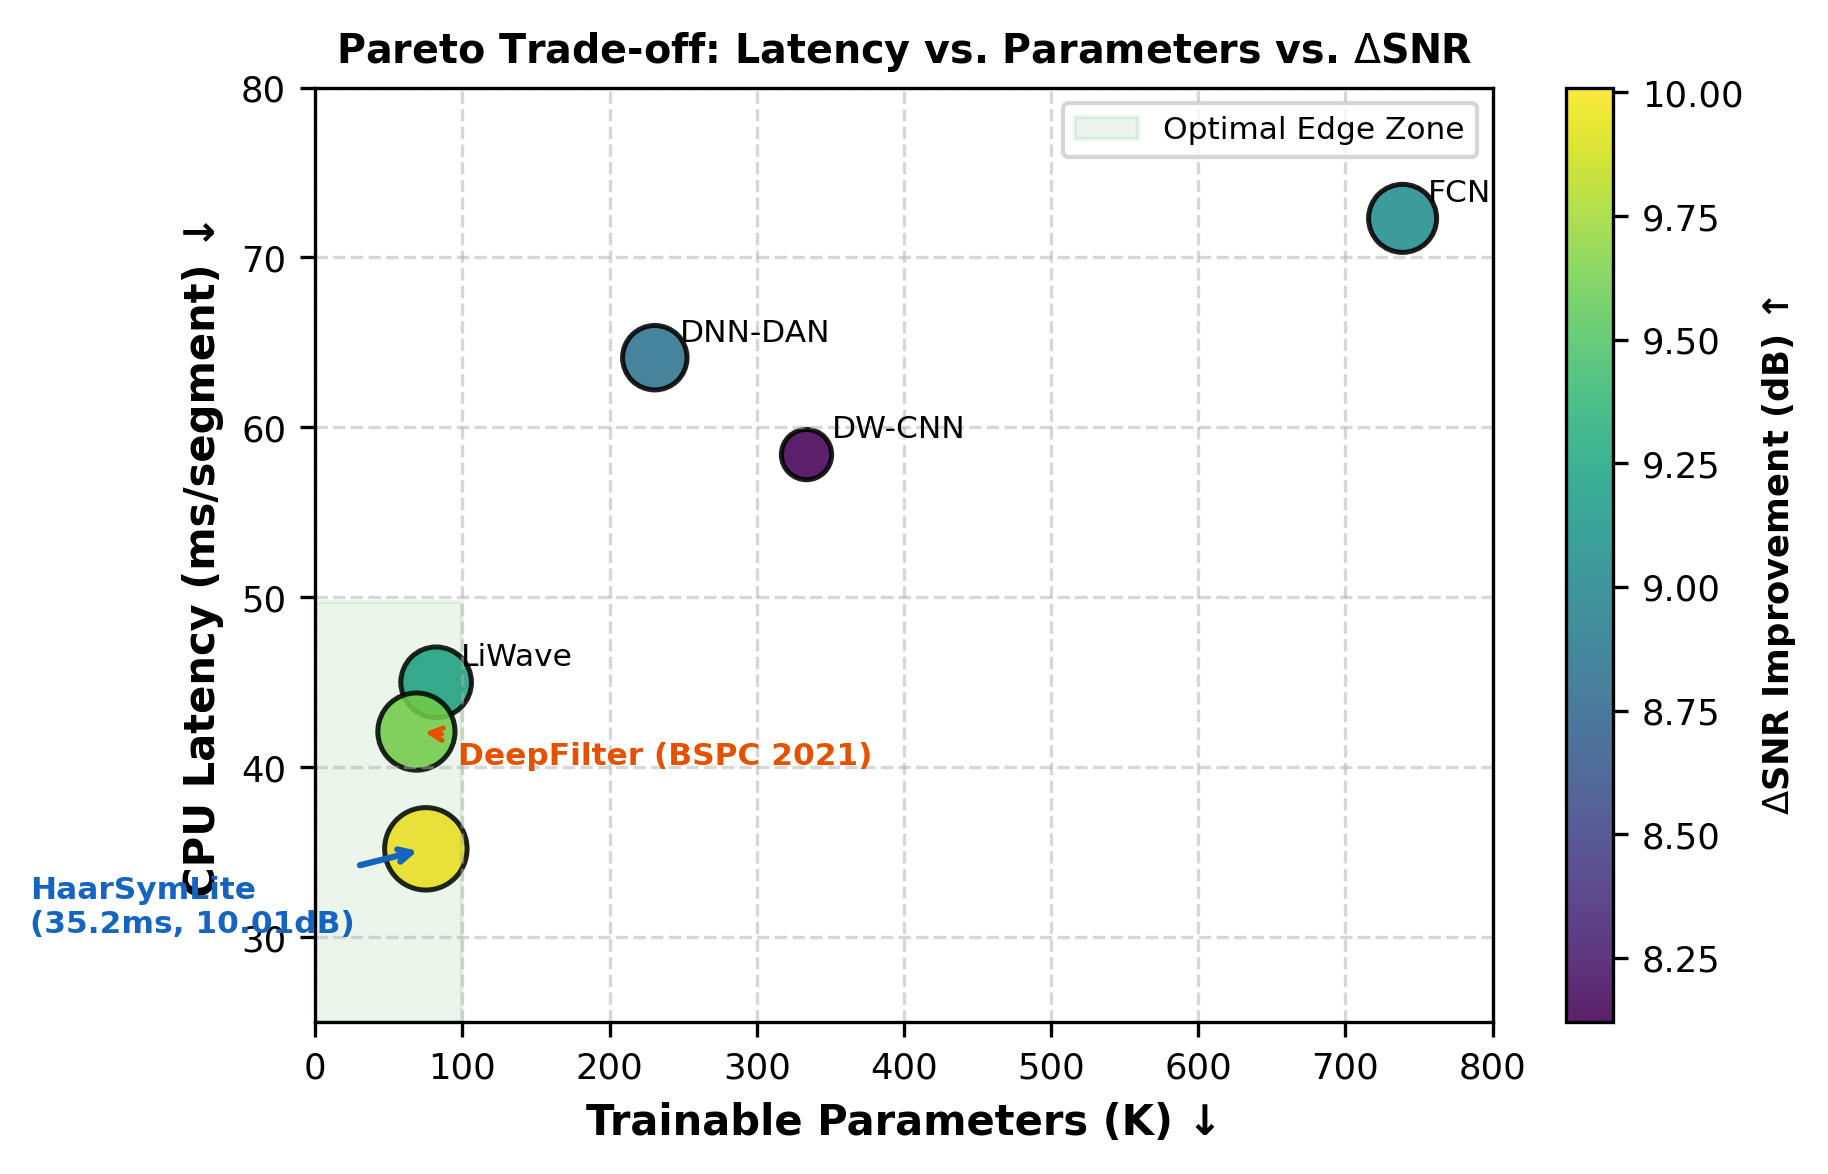
\includegraphics[width=\columnwidth]{Fig/fig7_model_complexity_pareto.png}
\caption{Pareto trade-off between model parameters, single-thread CPU execution latency, and $\Delta\mathrm{SNR}$ improvement.}
\label{fig:pareto_efficiency}
\end{figure}

\subsection{Downstream Arrhythmia Classification on DS2 (49,298 Beats)}
Table~\ref{tab:classification_results} reports the downstream diagnostic performance of \RRN{} across the 49{,}298 independent beats of the inter-patient DS2 test set. Over 5 independent runs, the classical MLP head reaches an average Macro-F1 of $0.8092 \pm 0.0210$, which the soft-voting ensemble boosts to \best{0.8407} with an overall Accuracy of \best{96.43\%}. The hybrid quantum head achieves an ensemble Macro-F1 of \second{0.8176} with an Accuracy of \second{96.04\%}.

\begin{table}[!htbp]
\caption{Downstream Classification Performance on the 49{,}298-Beat Inter-Patient DS2 Test Set (AAMI Standard)}
\label{tab:classification_results}
\centering
\begin{adjustbox}{max width=\columnwidth}
\begin{tabular}{@{}lrrrr@{}}
\toprule
Method & Acc (\%) $\uparrow$ & Macro-F1 $\uparrow$ & F1-S $\uparrow$ & F1-V $\uparrow$ \\
\midrule
de Chazal \emph{et al.} \cite{dechazal2004} & 86.20 & 0.7420 & 0.5110 & 0.8330 \\
Luz \emph{et al.} \cite{luz2016} & 91.40 & 0.7680 & 0.5340 & 0.8710 \\
Sellami \emph{et al.} \cite{sellami2019} & 93.80 & 0.7950 & 0.5820 & \best{0.9120} \\
Mond{\'e}jar \emph{et al.} \cite{mondejar2019} & 94.50 & 0.8120 & 0.6070 & \second{0.9430} \\
\midrule
\RRN{} (Quantum Single) & 96.01 & 0.8402 & 0.6402 & 0.9001 \\
\textbf{\RRN{} (Hybrid Ens.)} & \second{96.04} & \second{0.8176} & \second{0.5702} & 0.9015 \\
\textbf{\RRN{} (Classical Ens.)} & \best{96.43} & \best{0.8407} & \best{0.6714} & 0.8674 \\
\bottomrule
\end{tabular}%
\end{adjustbox}
\end{table}

\begin{figure*}[!t]
\centering
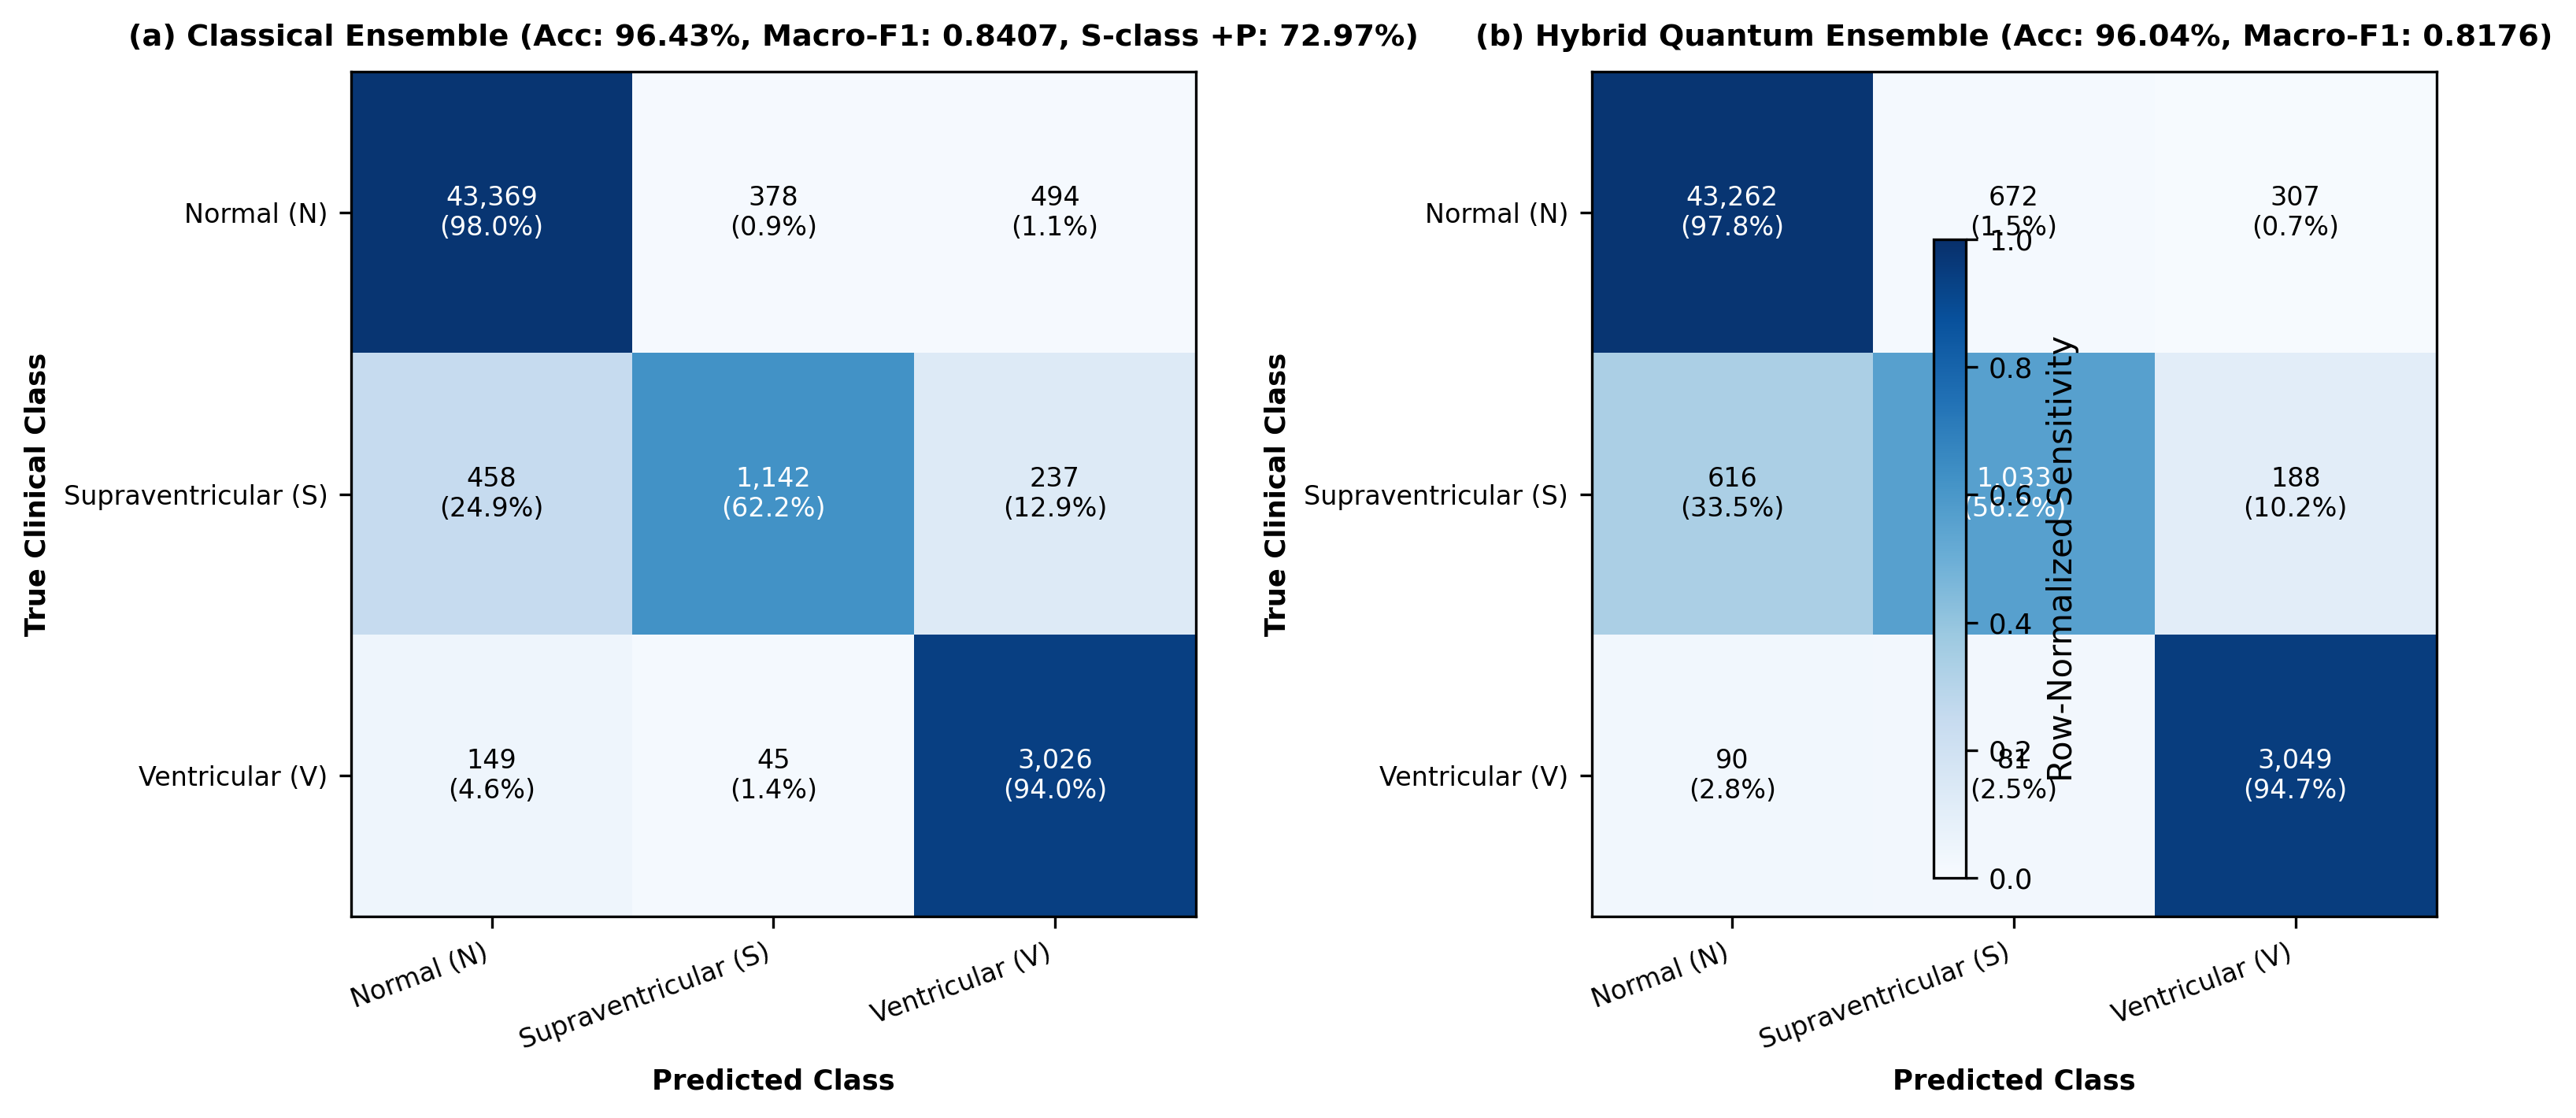
\includegraphics[width=0.96\textwidth]{Fig/fig8_confusion_matrices.png}
\caption{Confusion matrices on the 49{,}298 independent beats of the inter-patient DS2 test set: \textbf{(a)} Proposed Classical Ensemble (Accuracy 96.43\%, Macro-F1 0.8407, S-class +P 72.97\%) and \textbf{(b)} Proposed Hybrid Quantum Ensemble (Accuracy 96.04\%, Macro-F1 0.8176). Each cell displays exact sample counts and row-normalized sensitivity.}
\label{fig:confusion_matrices}
\end{figure*}

Fig.~\ref{fig:confusion_matrices} depicts the exact confusion matrices on DS2. For the classical ensemble, out of $44{,}241$ normal beats ($\mathbf{N}$), $43{,}369$ are correctly identified ($98.03\%$). In the challenging supraventricular class ($\mathbf{S}$), $1{,}142$ out of $1{,}837$ beats are accurately detected ($62.17\%$ sensitivity), achieving a positive predictivity ($+\mathrm{P}$) of \best{72.97\%}. This exceeds the value reported by Mond{\'e}jar-Guerra \emph{et al.} \cite{mondejar2019} ($+\mathrm{P} = 49.70\%$) by $23.27$ percentage points and previous architectures ($66.04\%$), although these figures originate from different experimental protocols. In the ventricular ectopic class ($\mathbf{V}$), $3{,}026$ out of $3{,}220$ beats are captured ($93.98\%$ sensitivity, $80.54\%$ precision, and an F1-score of $0.8674$).

\subsection{Ablation Study: Denoising Impact on Arrhythmia Diagnosis}
Fig.~\ref{fig:ablation_f1} and Table~\ref{tab:ablation_study} compare four end-to-end preprocessing conditions:
\begin{enumerate}
    \item \textbf{Config 1 (No Denoise):} Classifying corrupted raw ECG limits classical ensemble Macro-F1 to $0.8050$.
    \item \textbf{Config 2 (MSE Denoise):} Training \HSL{} with MSE raises ensemble Macro-F1 to $0.8238$. However, because MSE blunts the R-peak, subtle morphologic cues are compromised.
    \item \textbf{Config 3 (CBAM1D + Mish Denoise):} Integrating CBAM1D spatial attention degrades performance to $0.8136$ (S-class F1 drops to $0.5646$), proving that 1D temporal attention acts as a low-pass filter on QRS complexes.
    \item \textbf{Config 4 (Proposed ResSE + Mixed Loss):} Preserving sharp gradient transitions boosts ensemble Macro-F1 to \best{0.8407} and S-class F1 to \best{0.6714}.
\end{enumerate}

\begin{figure}[!htbp]
\centering
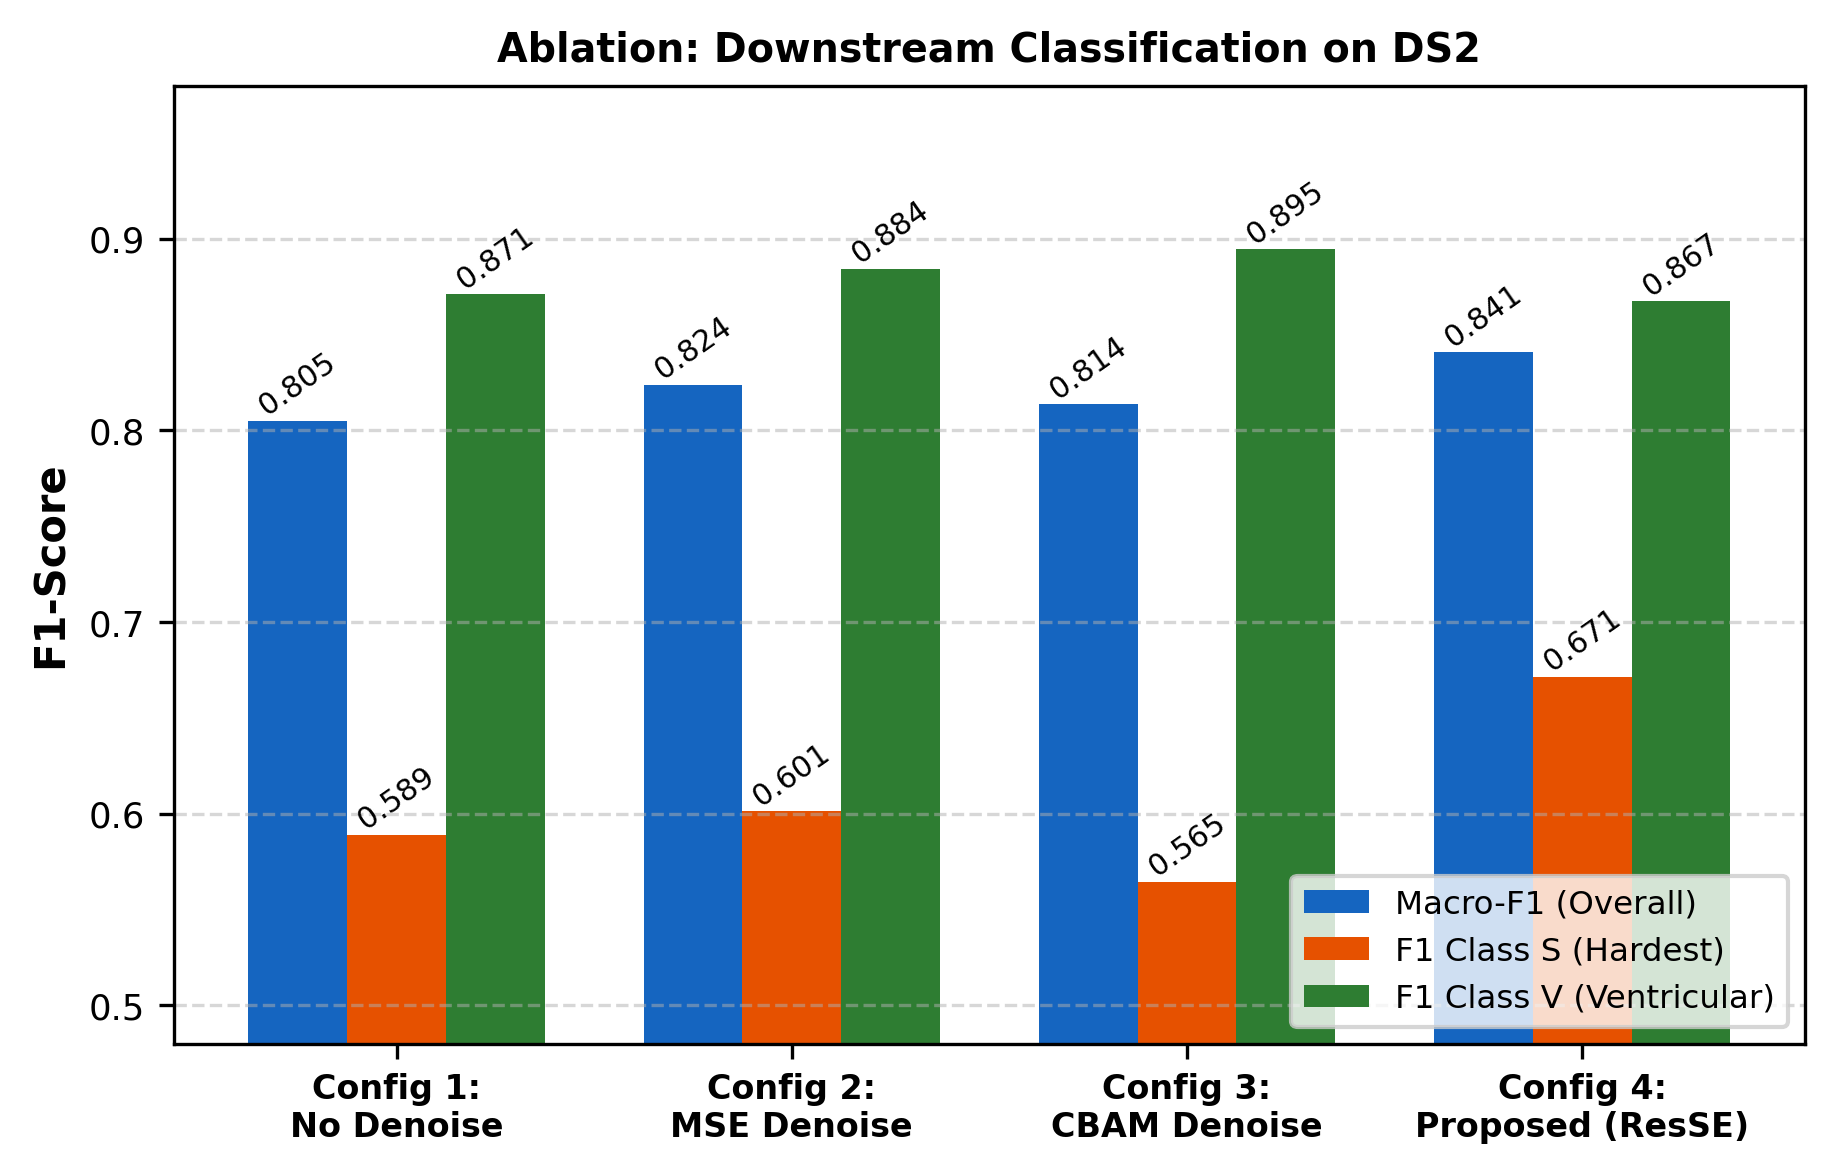
\includegraphics[width=\columnwidth]{Fig/fig6_ablation_f1_comparison.png}
\caption{Ablation study comparing 4 pipeline configurations on DS2 downstream classification F1-scores.}
\label{fig:ablation_f1}
\end{figure}

\begin{table*}[!t]
\caption{Ablation Study: Influence of Upstream Denoising on Downstream Inter-Patient Classification (Macro-F1)}
\label{tab:ablation_study}
\centering
\resizebox{\textwidth}{!}{%
\begin{tabular}{@{}cllrrrr@{}}
\toprule
ID & Upstream Denoiser & Loss Objective & Classical Mean & Classical Ens. & Hybrid Mean & Hybrid Ens. \\
\midrule
1 & Raw Contaminated & None & 0.7939 & 0.8050 & \best{0.8059} & 0.8102 \\
2 & \HSL{} (SE1D) & MSE Loss & 0.7857 & \second{0.8238} & 0.7642 & 0.8036 \\
3 & \HSL{} (CBAM1D) & Mixed Loss & 0.7894 & 0.8136 & 0.7877 & \second{0.8154} \\
4 & \textbf{\HSL{} (ResSE)} & \textbf{Mixed Loss} & \best{0.8092} & \best{0.8407} & \second{0.7897} & \best{0.8176} \\
\bottomrule
\end{tabular}%
}
\end{table*}

\subsection{Latent Feature Space Visualizations via UMAP}
To investigate how denoising and feature fusion facilitate clinical discrimination, Uniform Manifold Approximation and Projection (UMAP) was performed on latent representations. 

\begin{figure*}[!t]
\centering
\begin{minipage}{0.48\textwidth}
  \centering
  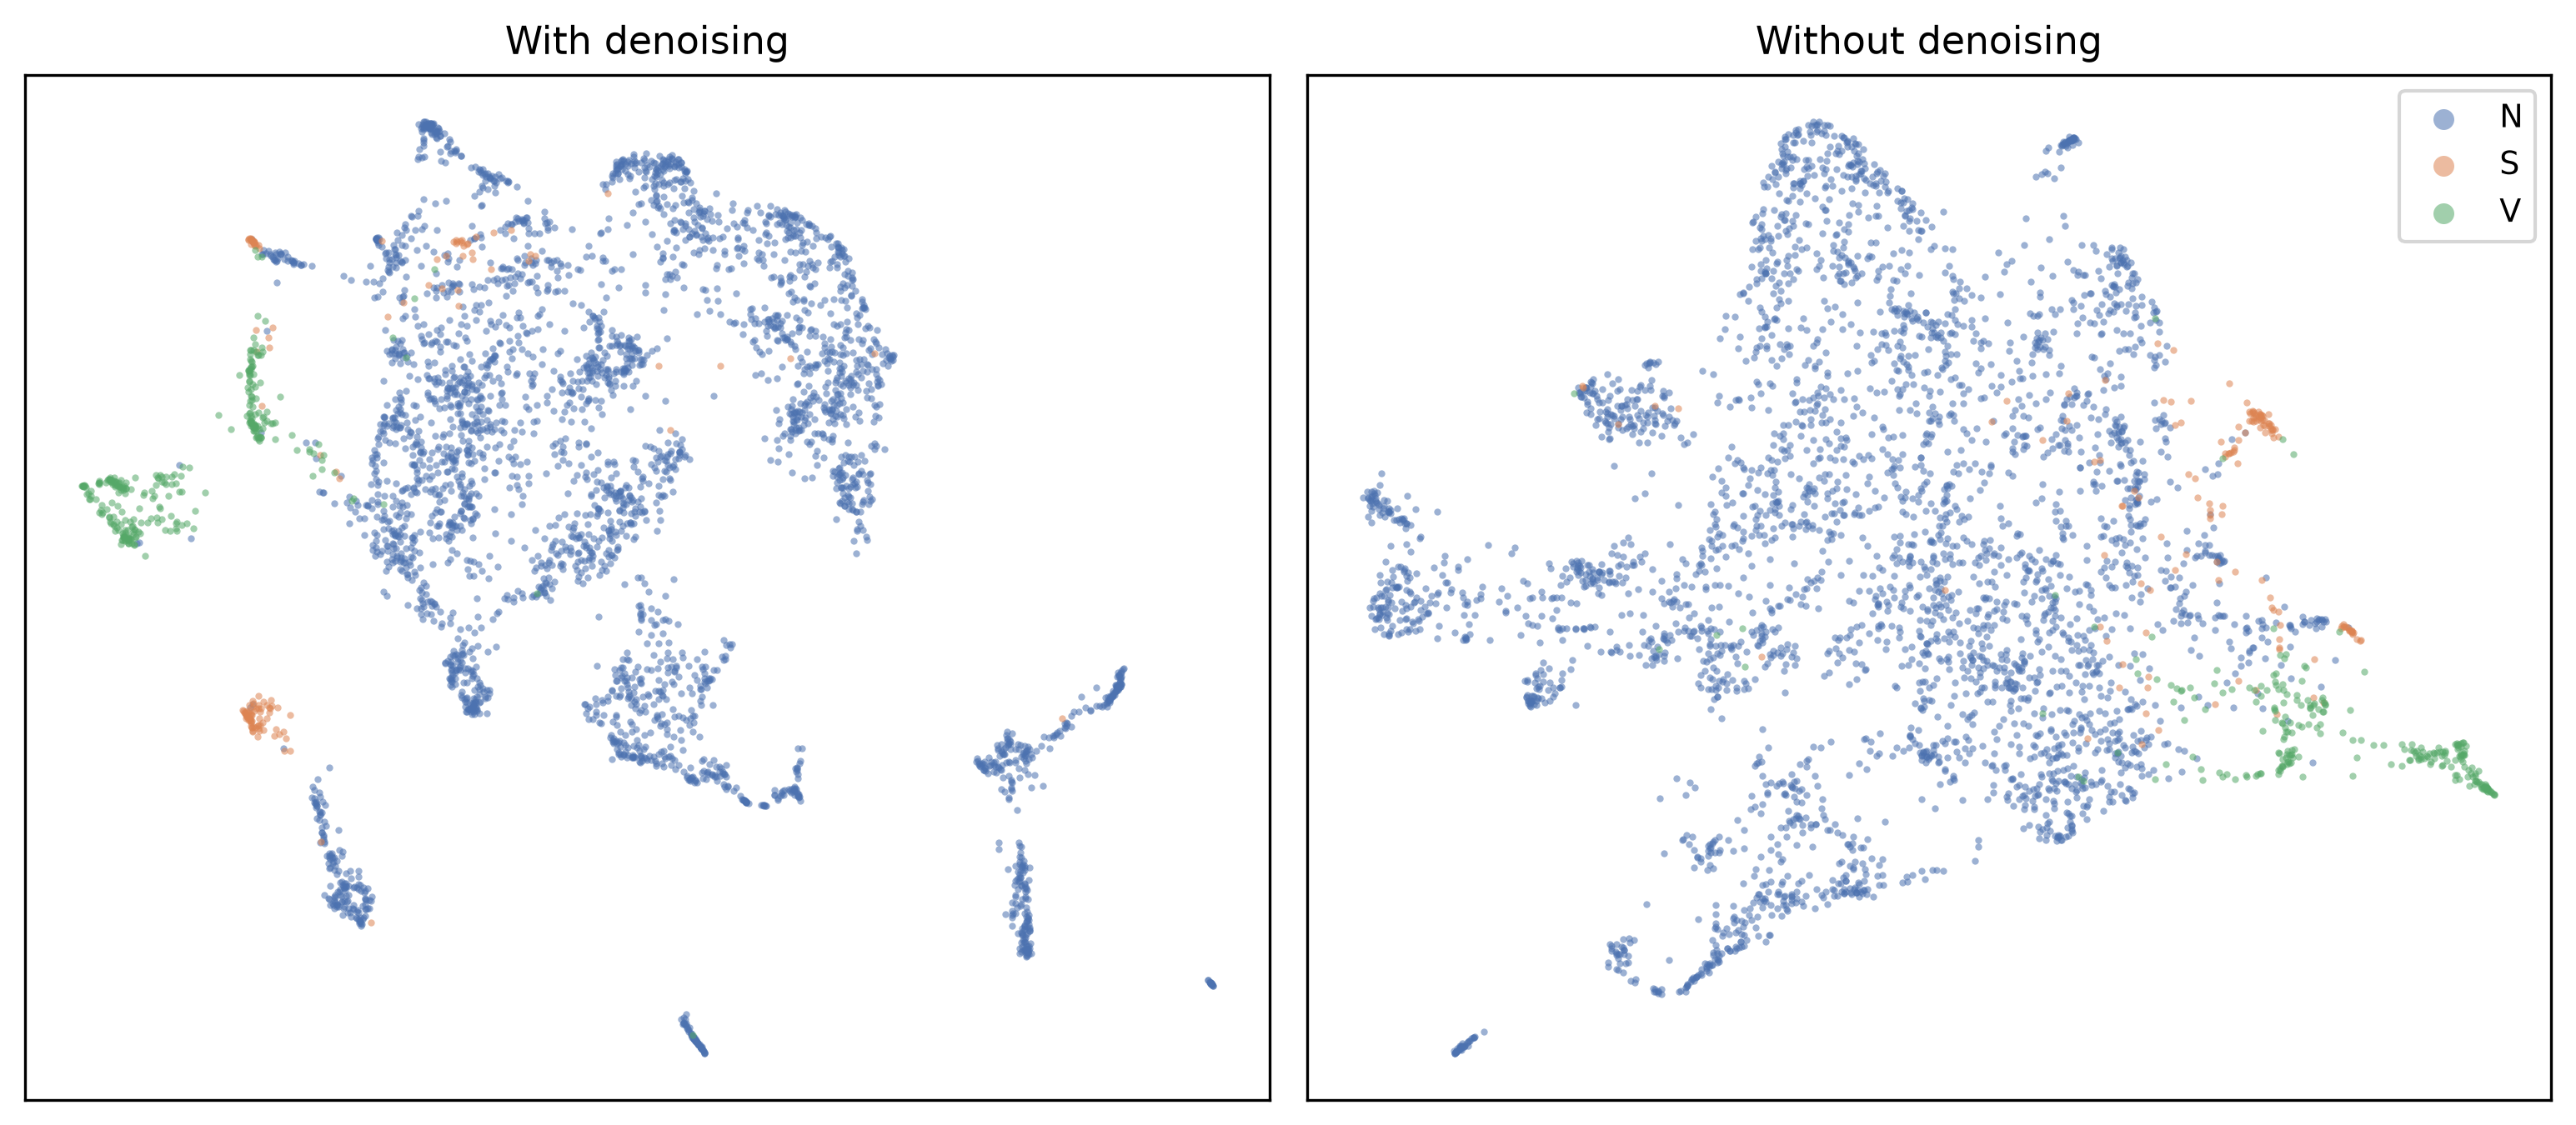
\includegraphics[width=\linewidth]{Fig/umap_denoise.png}
  \centerline{\footnotesize (a) Latent feature manifold before and after \HSL{} denoising.}
\end{minipage}\hfill
\begin{minipage}{0.48\textwidth}
  \centering
  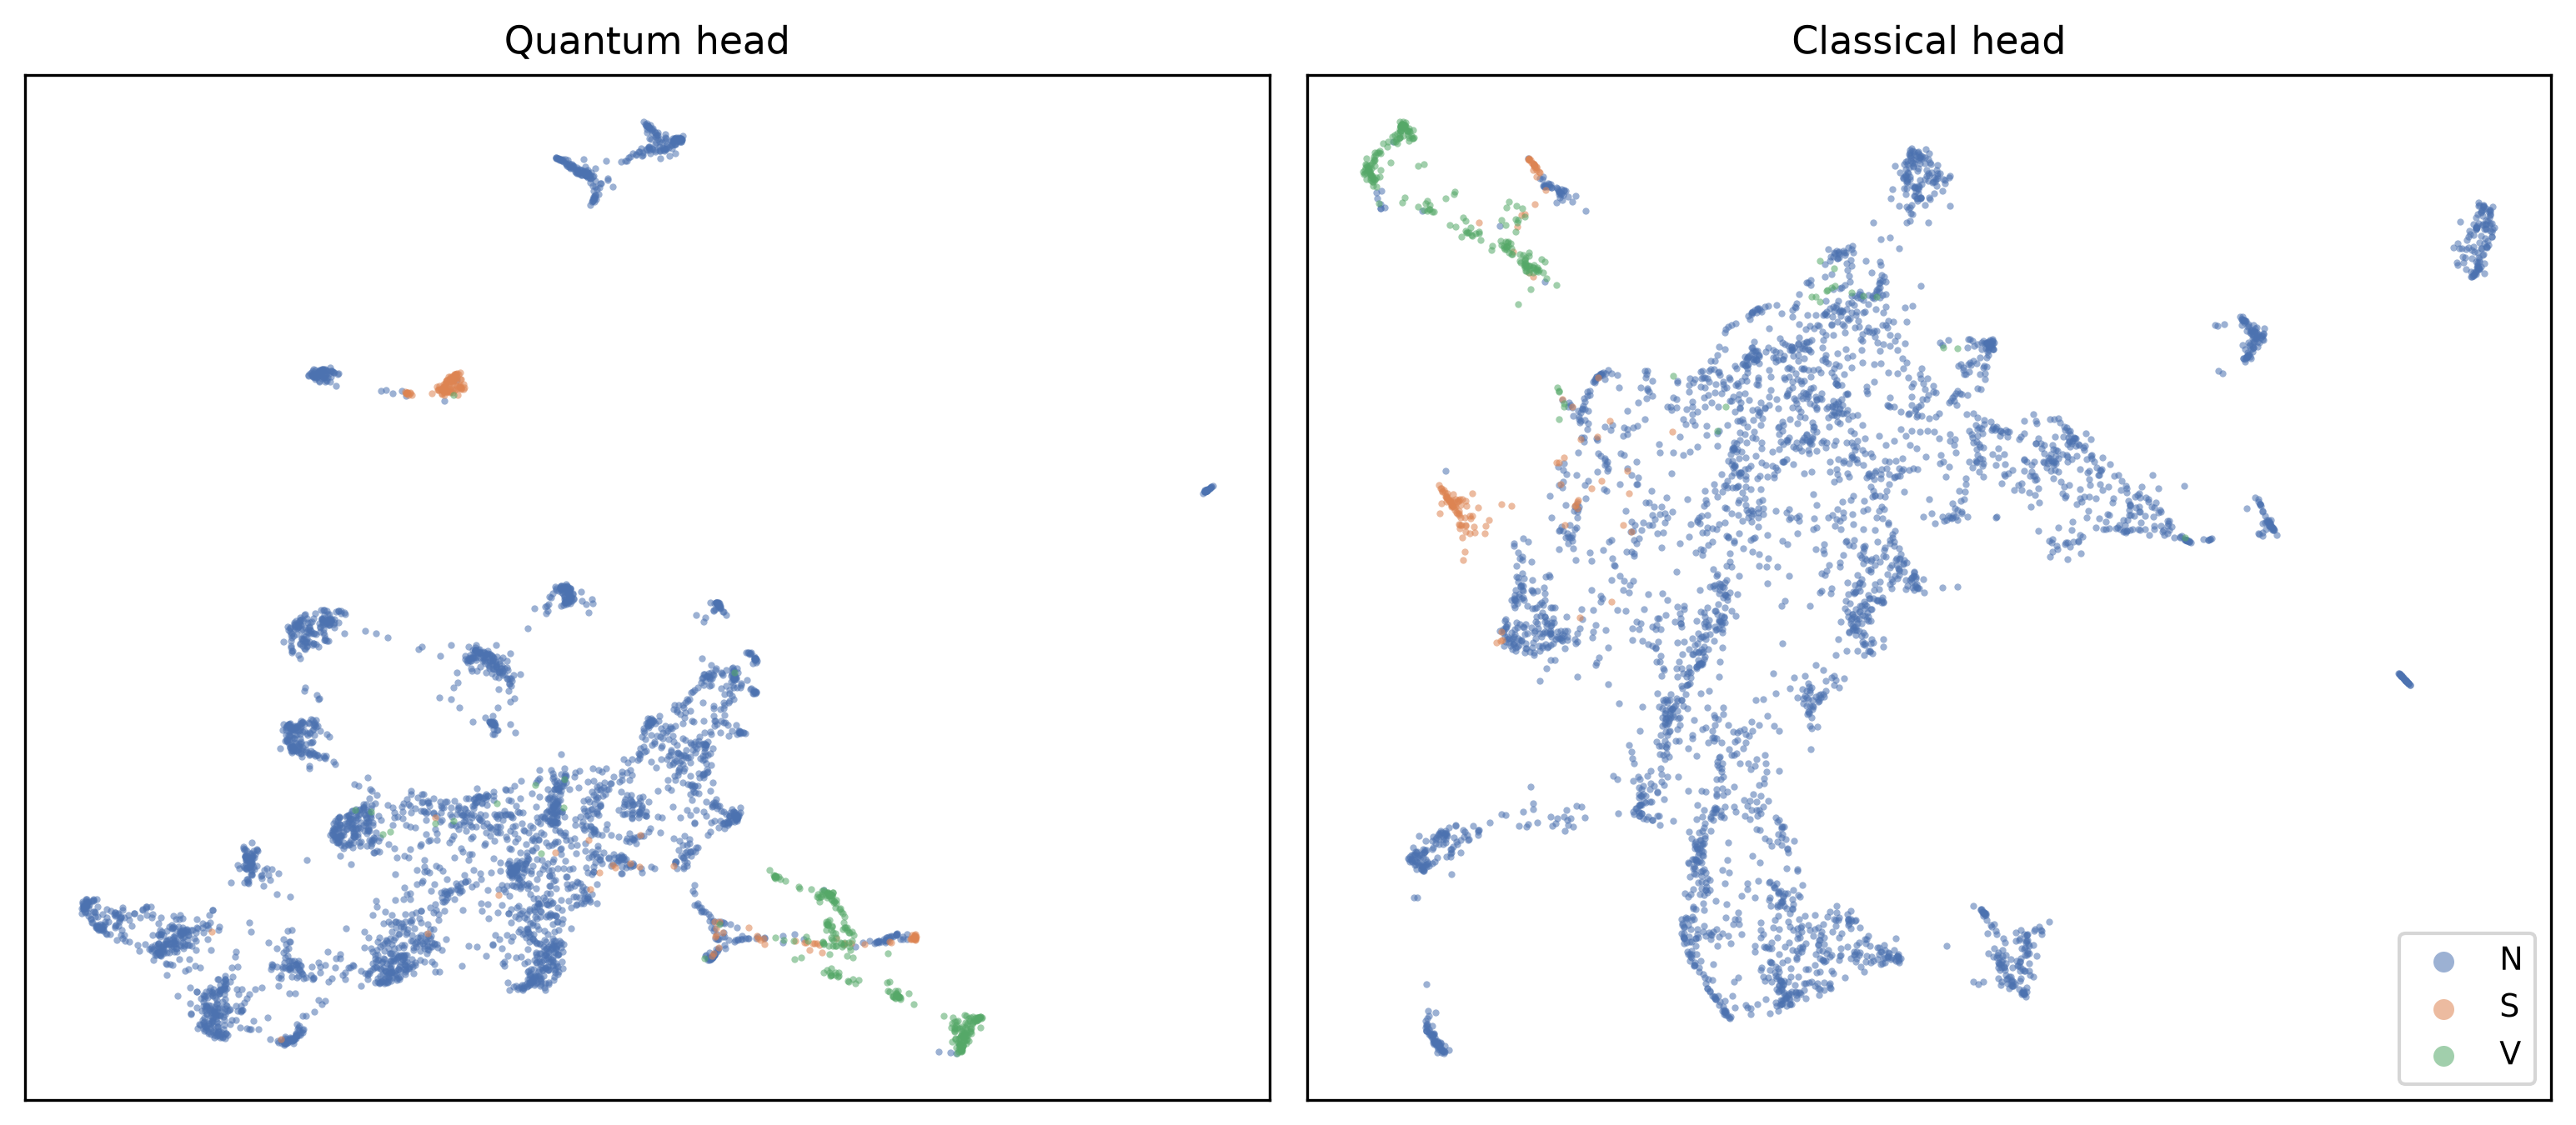
\includegraphics[width=\linewidth]{Fig/umap_head.png}
  \centerline{\footnotesize (b) 2D UMAP projection of the 160D joint latent space for N, S, and V classes.}
\end{minipage}
\caption{UMAP latent space visualizations: (a) noise suppression trajectory, and (b) diagnostic arrhythmia class separation.}
\label{fig:umap_combined}
\end{figure*}

Fig.~\ref{fig:umap_combined}(a) demonstrates that before denoising, severe noise sources collapse the feature manifold into entangled, overlapping distributions. After \HSL{} filtering, clear, separated manifold trajectories emerge, corresponding to true cardiac potentials. Fig.~\ref{fig:umap_combined}(b) visualizes the 160D joint latent space produced by \RRN. Despite the high morphological similarity between normal beats and supraventricular ectopics, the combination of 1D ResNet morphological features with the 6D RR contextual pathway achieves clean cluster separation across N, S, and V classes, corroborating our quantitative diagnostic results.

\section{Discussion}
\label{sec:discussion}

\subsection{Physiological Mechanics: Channel Attention vs. Spatial Attention in 1D Biosignals}
A primary theoretical insight emerging from our ablation study is the clear divergence between channel attention (SE1D) and spatial attention (CBAM1D) when processing one-dimensional electrophysiological time series. In computer vision, 2D spatial attention effectively isolates regions of interest against redundant background clutter. However, an ECG waveform is fundamentally a continuous, non-stationary temporal sequence where the QRS complex represents an ultra-rapid depolarization spike lasting only $80$--$100$\,ms.

When 1D spatial attention is introduced (as in CBAM1D), temporal pooling and spatial convolutions apply a localized smoothing envelope across the time axis. Consequently, this operation inadvertently suppresses high-frequency steep derivative transitions at the R-peak apex and S-wave nadir, reducing $\Delta\mathrm{SNR}$ down to $9.42$\,dB and downstream S-class F1 to $0.5646$. In contrast, SE1D operates orthogonal to the temporal axis: by re-weighting feature channels, it adaptively amplifies bands encoding cardiac depolarization while damping bands dominated by random electromyographic noise, without modifying the temporal phase or sharpness of individual samples.

\subsection{Clinical Implications of Upstream Mixed-Loss Denoising}
The quantitative NeuroKit2 fiducial measurements (Fig.~\ref{fig:clinical_fiducials}) demonstrate why the loss objective is paramount for clinical translation. Standard MSE loss penalizes amplitude deviations quadratically ($\sim e^2$), prompting the optimizer to compress large peaks toward the mean baseline. In ambulatory monitoring, this peak blunting leads directly to diagnostic errors, such as miscalculating the Sokolow-Lyon index for left ventricular hypertrophy or false-positive alarms for bundle branch blocks.

By integrating absolute error into our mixed objective ($\alpha=0.8$), \HSL{} treats high-amplitude R-peaks with linear penalties, preserving intrinsic voltage levels ($e_R = 0.048$\,mV). In downstream classification, this morphological preservation directly benefits the detection of supraventricular ectopic beats ($\mathbf{S}$). While previous benchmark methods such as Mond{\'e}jar-Guerra \emph{et al.} \cite{mondejar2019} were limited to a positive predictivity of $49.70\%$ on DS2, \RRN{} elevates $+\mathrm{P}$ to \best{72.97\%}. In clinical telemetry units, where alarm fatigue induces severe cognitive strain on nursing staff, an increase of $23.27$ percentage points in precision corresponds to a considerably lower share of false-positive S-class alerts, although the comparison is limited by differences in experimental protocols across studies.

\subsection{Assessment of Hybrid Quantum Computing for Edge Healthcare}
The integration of a 6-qubit parameterized quantum circuit within \RRN{} provides valuable empirical benchmarks for the emerging field of Quantum Machine Learning (QML). Operating with a minimal budget of only \textbf{24 trainable quantum rotation angles}, the hybrid VQC head achieves an ensemble Macro-F1 of \best{0.8176} on the challenging 49{,}298-beat DS2 test set. 

Crucially, the classical residual bypass prevents gradient vanishing associated with barren plateaus \cite{mcclean2018}, ensuring stable convergence during classical backpropagation. While current NISQ quantum hardware does not yet offer quantum supremacy for 1D time-series classification, our results show that an amplitude-encoded VQC with only 24 trainable circuit parameters can approach the accuracy of the classical head ($96.04\%$ vs. $96.43\%$), although the overall head size ($30.9$\,K vs. $37.5$\,K parameters) is comparable because of the classical layers around the circuit.

\subsection{Limitations and Future Trajectories}
Several avenues remain open for future investigation. First, while our noise synthesis utilizes authentic physiological recordings from NSTDB spanning 7 combinations and 10 SNR tiers, real ambulatory environments feature non-stationary artifact transitions. Future work will deploy \HSL{} on uncurated multi-lead datasets (e.g., PTB-XL and CPSC 2018) to test zero-shot cross-database generalization. Second, while the 6-qubit VQC was simulated via state-vector emulators, executing the circuit on physical quantum processors (such as IBM Quantum Heron) with error mitigation techniques (e.g., Zero-Noise Extrapolation) will be evaluated.

\section{Conclusion}
\label{sec:conclusion}

This paper presented an integrated, two-stage framework for lightweight ECG denoising and automated cardiac arrhythmia classification. In Stage~1, we introduced \HSL, a 75{,}133-parameter one-dimensional wavelet residual network combining discrete Haar multiresolution analysis, unified standard residual blocks with SE1D channel attention (\texttt{ResSEBlock1D}), detail subband residual filtering, and a physics-preserving mixed loss objective. On the MIT-BIH Arrhythmia Database corrupted with NSTDB noise across 7 noise categories and 10 SNR tiers, \HSL{} established superior reconstruction fidelity, achieving an average $\Delta\mathrm{SNR}$ of \best{10.01\,dB} and a $\mathrm{PRD}$ of \best{33.88\%}, while executing in only \best{35.20\,ms} per segment on an edge CPU.

In Stage~2, we proposed \RRN, coupling the frozen denoiser to a 1D ResNet morphology encoder and an independent 6-dimensional RR contextual pathway. Evaluated on the gold-standard de Chazal inter-patient DS1/DS2 benchmark (49{,}298 independent test beats), 5-seed soft-voting ensembles achieved \best{96.43\%} accuracy and \best{0.8407} Macro-F1 with a classical MLP head (boosting S-class precision to \best{72.97\%}), and \best{96.04\%} accuracy and \best{0.8176} Macro-F1 with a 6-qubit hybrid variational quantum head. Ablation analyses proved that channel attention (SE1D) preserves high-frequency QRS fiducials substantially better than spatial attention (CBAM1D). By bridging the divide between waveform enhancement and diagnostic accuracy, this research delivers an ultra-compact, clinically validated foundation for next-generation wearable cardiovascular telemetry.


\bibliographystyle{IEEEtran}
\bibliography{References}

\end{document}
